% !TEX program = xelatex
% 任务一独立论文：白葡萄酒质量分类
\documentclass[12pt,a4paper,fontset=fandol]{ctexart}
\usepackage[a4paper,margin=2.4cm]{geometry}
\usepackage{graphicx}
\usepackage{booktabs}
\usepackage{multirow}
\usepackage{float}
\usepackage{caption}
\usepackage{array}
\usepackage{amsmath}
\usepackage{amssymb}
\usepackage{enumitem}
\usepackage{setspace}
\usepackage{hyperref}
\hypersetup{hidelinks}

\captionsetup{font=small, labelsep=quad}
\graphicspath{{./}{../../report/}{../../task1_ml_wine/outputs/}}
\renewcommand{\arraystretch}{1.3}
\setlength{\parindent}{2em}
\setlength{\emergencystretch}{3em}
\numberwithin{figure}{section}
\numberwithin{table}{section}
\numberwithin{equation}{section}
\onehalfspacing
\pagestyle{plain}

\ctexset{
  section/format = \zihao{4}\heiti\raggedright,
  section/beforeskip = {1ex plus 0.2ex},
  section/afterskip = {0.8ex plus 0.2ex},
  subsection/format = \zihao{-4}\heiti\raggedright,
  subsubsection/format = \zihao{-4}\kaishu\raggedright
}

\begin{document}

% ===================== 封面 =====================
\begin{titlepage}
\centering
\vspace*{1.5cm}
{\Large 本科毕业论文（设计）}\\[1.5cm]
{\Huge\bfseries 人工智能综合实训 II}\\[0.6cm]
{\LARGE\bfseries 任务一实训论文}\\[1.2cm]
{\Large\bfseries 传统机器学习模型对结构化数据分类性能的影响研究}\\[0.4cm]
{\large\bfseries ——以白葡萄酒质量分类为主线的多数据集实证}\\[2cm]
{\large
\renewcommand{\arraystretch}{1.7}
\begin{tabular}{rl}
\textbf{学\qquad 院：} & 人工智能与低空技术学院 \\
\textbf{专\qquad 业：} & 人工智能 \\
\textbf{小组成员：} & 雷正（202434610309）、蔡铭飞（202434610301）、 \\
                    & 冼嘉谦（202434610326） \\
\textbf{指导教师：} & 赵静 \\
\textbf{提交日期：} & 2026 年 6 月 \\
\end{tabular}}
\vfill
\end{titlepage}

% ===================== 原创性声明 =====================
\thispagestyle{empty}
\begin{center}{\large\bfseries 华南农业大学本科毕业论文（设计）原创性声明}\end{center}
\vspace{0.5em}
\par 本人郑重声明：所呈交的毕业论文（设计），是本人在导师的指导下，独立进行研究工作所取得的成果。
除文中已经注明引用的内容外，本论文不包含任何其他个人或集体已经发表或撰写过的作品成果。对本文的研究
做出重要贡献的个人和集体，均已在文中以明确方式标明。本人完全意识到本声明的法律结果由本人承担。
\vspace{1.2cm}
\par\hfill 作者签名：\rule{3cm}{0.4pt}\qquad 日期：\quad\ 年\ \quad 月\ \quad 日\hspace{1cm}
\vspace{2cm}

\begin{center}{\large\bfseries 华南农业大学本科毕业论文（设计）使用授权声明}\end{center}
\vspace{0.5em}
\par 本人完全了解学校有关保留、使用毕业论文（设计）的规定，同意学校保留并向国家有关部门或机构送交
毕业论文（设计）的复印件和电子版，允许毕业论文（设计）被查阅和借阅。学校可以将本毕业论文（设计）的
全部或部分内容编入有关数据库进行检索，可以采用影印、缩印或扫描等复制手段保存和汇编毕业论文（设计）。
\vspace{1.2cm}
\par\hfill 作者签名：\rule{3cm}{0.4pt}\qquad 指导教师签名：\rule{3cm}{0.4pt}\hspace{1cm}
\par\hfill 日期：\quad\ 年\ \quad 月\ \quad 日\qquad\quad 日期：\quad\ 年\ \quad 月\ \quad 日\hspace{1cm}
\newpage

% ===================== 摘要 =====================
\begin{center}{\Large\bfseries 摘\quad 要}\end{center}
\par 结构化数据分类是机器学习的典型问题。本文\textbf{以支持向量机、决策树、随机森林和逻辑回归四种
代表性模型为研究对象}，以 UCI Wine Quality 数据集中的白葡萄酒子集为主实验平台，将原始质量评分归并为
“差”“中”“好”三类，围绕数据加载、探索性分析、预处理、模型构建、模型评估和结果分析完成完整机器
学习流程，并采用标准化流水线、五折交叉验证和网格搜索进行超参数选择；在此基础上，进一步把同一套模型
推广到难度递增的五个结构化数据集上对照，并对其中表现欠佳者做针对性处理，考察数据特点与模型选择如何
共同决定性能。

\par 实验结果表明，随机森林在测试集上取得较优表现，准确率为 73.47\%，宏平均 F1 为 0.7336；在平衡
准确率、二次加权 Kappa、MCC 和宏平均 ROC-AUC 等进阶指标上也表现较好。进一步的混淆矩阵分析显示，
模型误差主要集中于相邻质量等级之间，严重跨级误判较少。基于这一特点，本文补充采用“回归预测质量分
再分级”的有序建模方式进行对照，结果显示宏平均 F1 由 0.7336 提升至 0.7533，严重跨级误判数由 7 降至
4。整体来看，集成学习方法适合该类中小规模结构化数据分类任务，而显式关注标签顺序有助于改进质量
等级预测的误差结构。

\par 跨数据集对照进一步表明：不存在放之四海而皆准的最优模型，最优选择随数据集而变；类别数量并非主要
难度来源；极端类别不平衡会使准确率严重失真，须以宏平均 F1 或平衡准确率衡量。针对表现欠佳的贷款违约与
臭氧数据，本文先以补充申请时类别特征、SMOTE 过采样和更换更强模型（GBDT）等静态手段验证，宏平均 F1 均
停留在约 0.58 至 0.62；进而从任务本身出发设计针对性创新——把臭氧从“无序表格”还原为时间序列并注入时序
特征、为贷款违约补全数十个真实征信特征并注入信用评分领域单调约束。值得强调的是，臭氧时序特征在\emph{单次}
时序划分下一度呈现 +0.058 的宏 F1 提升，但因该划分测试集仅含约 4 个少数类样本而高度不可靠；改用时序交叉
验证汇集约 58 个少数类样本后，该提升消失（$\Delta\approx-0.003$）；而为贷款违约补入数十个真实征信特征后宏
平均 F1 仍仅由 0.585 变为 0.586，单调约束亦持平于约 0.57。这表明两个数据集的“效果不好”确属弱判别信号或极端
不平衡的数据本质——即便补全真实信息也几乎无增益（因利率已是征信信息的近似充分统计量）；同时给出一条评估
方法学教训：极端不平衡下须以交叉验证汇集足够少数类样本，方能避免单次划分造成的“假提升”。

\par\vspace{1ex}
\noindent\textbf{关键词：}机器学习；结构化数据分类；模型对照；类别不平衡；时序交叉验证；单调约束；跨数据集

\newpage
\begin{center}{\Large\bfseries Abstract}\end{center}
\par Wine quality prediction is a representative structured-data classification problem. This paper studies the
white wine subset of the UCI Wine Quality dataset. The original quality scores are merged into three classes:
low, medium and high. A complete machine learning workflow is implemented, including data loading, exploratory
analysis, preprocessing, model construction, model evaluation and result analysis. Four representative classifiers,
including support vector machine, decision tree, random forest and logistic regression, are compared using a
standardized pipeline, five-fold cross validation and grid search.

\par The experimental results show that random forest achieves relatively better performance on the test set, with
an accuracy of 73.47\% and a macro-F1 score of 0.7336. It also performs well on balanced accuracy, quadratic
weighted Kappa, MCC and macro ROC-AUC. Further analysis of the confusion matrix indicates that most errors occur
between adjacent quality levels, while severe cross-level errors are rare. Based on this observation, a
regression-then-discretization strategy is evaluated as an additional ordinal modeling comparison. The macro-F1
score increases from 0.7336 to 0.7533, and the number of severe cross-level errors decreases from 7 to 4. Overall,
ensemble learning is suitable for this medium-sized structured-data classification task, and explicitly considering
the order of labels helps improve the error structure of wine quality prediction.

\par\vspace{1ex}
\noindent\textbf{Keywords:} machine learning; white wine quality; support vector machine; random forest; ordinal modeling; multi-class classification

\newpage
\tableofcontents
\newpage

% ===================== 第一章 引言 =====================
\section{引言}

\subsection{研究背景与意义}
结构化数据分类是机器学习应用中最常见的任务之一，广泛存在于食品质量评价、金融风险判断、医学辅助诊断
和业务决策等场景。与图像、文本等非结构化数据不同，结构化数据通常由仪器测量、业务记录或人工标注得到，
具有特征含义明确、维度相对有限、样本规模中等、噪声来源可解释等特点。对于这类数据，深度学习并不总是
最优或最经济的选择，支持向量机、决策树、随机森林、逻辑回归等传统机器学习方法仍然具有训练成本低、调试
方便、结果较易解释等优势。

葡萄酒质量评价兼具实际应用价值和方法研究价值。在真实生产场景中，葡萄酒质量通常受到酸度、糖分、硫化物、
密度、酒精度等多种理化因素影响，最终评分又带有一定主观性。若能够基于理化指标建立稳定的质量分级模型，
可以辅助质量控制、产品筛选和生产工艺分析。Cortez 等(2009)整理的 Wine Quality 数据集将理化检测指标与
质量评分对应起来，为研究化学属性与感官质量之间的统计关系提供了公开基准。

该任务的难点在于，葡萄酒质量评分并不是完全离散、边界清晰的类别标签。一方面，数据集中样本主要集中在
中间分值，极高和极低评分样本较少，类别分布不均衡会影响模型训练和评价；另一方面，质量评分具有天然顺序，
相邻等级之间的误判和跨等级误判在实际含义上并不相同。若只采用总体准确率评价模型，容易忽略少数类别表现
和误差等级距离。因此，本研究不仅比较多种传统分类模型的性能，还进一步引入宏平均 F1、二次加权 Kappa、
有序 MAE 和严重跨级误判数等指标，从误差结构角度讨论质量分级模型的适用性。

从实训和研究方法角度看，白葡萄酒质量分类任务能够覆盖结构化数据建模的完整流程，包括数据读取与查看、
探索性分析、标签构造、标准化、交叉验证、模型选择、测试集评价和结果解释。通过该任务，可以较系统地理解
传统机器学习在中小规模结构化数据上的建模思路，并分析不同模型在可解释性、泛化能力和错误类型上的差异。

\subsection{国内外研究现状}
围绕结构化分类任务，国内外研究已经形成了较成熟的方法体系。周志华(2016)从监督学习、模型选择和泛化能力
等角度系统总结了传统机器学习方法，为结构化数据分类提供了基础理论框架。逻辑回归作为广义线性模型的代表，
具有参数含义清晰、训练效率高等特点，常用于建立可解释的分类基线。支持向量机由 Cortes 和 Vapnik(1995)
提出，通过最大间隔原则提高分类器泛化能力，并可借助核函数刻画非线性边界，在中小规模数据集上具有较强
竞争力。

树模型及其集成方法是结构化数据建模中的重要方向。单棵决策树能够形成较直观的特征划分规则，但对训练样本
扰动较敏感，容易产生较高方差。Breiman(2001)提出随机森林，通过 Bootstrap 采样、随机特征选择和多树投票
降低方差，在表格数据任务中具有较好的稳定性。此后，梯度提升树进一步通过逐步拟合残差提升预测能力，
XGBoost 和 LightGBM 等方法在工程效率和预测性能方面得到广泛应用。由于本文重点在于比较典型传统分类器并
完成完整建模流程，实验主体选择了逻辑回归、支持向量机、决策树和随机森林，其中随机森林兼具非线性表达和
一定可解释性，适合与葡萄酒理化指标任务相结合。

葡萄酒质量预测方面，Cortez 等(2009)以红葡萄酒和白葡萄酒理化检测数据为基础，研究了数据挖掘方法对感官
偏好建模的可行性。该数据集被广泛用于分类、回归、特征重要性分析和模型比较。已有研究通常关注理化指标与
质量评分之间的统计关联，其中酒精度、挥发性酸度、密度等变量常被认为与质量判断关系较密切。由于原始质量
分值集中在少数等级，直接进行多分值分类容易受到少数类样本不足影响，因此不少实验会将原始评分合并为二类
或三类，以获得更稳定的训练和评价结果。

类别不平衡和有序标签是该任务中需要重点处理的两个问题。He 和 Garcia(2009)指出，不平衡学习中总体准确率
可能掩盖少数类别识别效果，因此需要结合平衡准确率、F1、MCC 等指标进行评价。另一方面，McCullagh(1980)
提出的有序回归思想强调类别之间存在顺序关系时，模型和评价指标应区分不同等级距离的误差。葡萄酒质量评分
从低到高具有明确次序，将其完全视为无序类别会弱化相邻误判与严重跨级误判之间的差异。因此，本文在常规
三分类实验之外补充有序回归分级对照，并引入二次加权 Kappa 和严重误判数，以更贴合质量分级任务的实际语义。

\subsection{研究内容与分工}
本文\textbf{以四种传统机器学习模型为研究对象}，以白葡萄酒质量三分类为主线，把数据集视为检验模型的
试验台。主要工作包括两个层面：其一，在白葡萄酒数据上完成加载与查看、三分类标签构造、特征标准化与
分层划分、四种模型训练与网格搜索、测试集指标评价、混淆矩阵与特征重要性分析，以及基于误差结构的有序
建模补充实验；其二，将同一套建模管线推广到难度递增的五个结构化数据集上对照，并对其中表现欠佳的数据集
做针对性处理（补充特征、不平衡重采样），分析数据特点与模型选择如何共同决定性能。小组成员分工如
表~\ref{tab:team} 所示。

\begin{table}[H]
  \centering
  \caption{小组成员分工表}
  \label{tab:team}
  \begin{tabular}{>{\centering\arraybackslash}m{3cm} >{\centering\arraybackslash}m{2cm} m{8cm}}
    \toprule
    学号 & 姓名 & 主要分工 \\
    \midrule
    202434610301 & 蔡铭飞 & 数据预处理、四种模型训练与网格搜索、跨数据集对照与不平衡/特征改进实验、结果评估 \\
    202434610309 & 雷正 & 总体方案设计、实验结果分析、论文主体撰写与复现说明整理 \\
    202434610326 & 冼嘉谦 & 数据可视化、图表绘制、论文排版、PPT 制作与汇报 \\
    \bottomrule
  \end{tabular}
\end{table}

% ===================== 第二章 理论基础与实验设计 =====================
\section{理论基础与实验设计}

\subsection{监督学习与多分类问题}
监督学习是在带标签训练集上学习从输入空间到输出空间的映射：
\begin{equation}
D=\{(\mathbf{x}_i,y_i)\}_{i=1}^{N},\qquad f:\mathcal{X}\rightarrow\mathcal{Y}.
\end{equation}
当标签取离散值时，该任务为分类问题。本文将白葡萄酒质量评分转化为三分类标签，即低质量、中等质量和高
质量。模型学习的目标是在训练数据上最小化损失函数，并在独立测试集上取得良好的泛化性能。

从经验风险最小化角度看，分类模型通常通过训练样本上的平均损失近似总体风险：
\begin{equation}
\hat{f}=\arg\min_{f\in\mathcal{F}}\frac{1}{N}\sum_{i=1}^{N}L\bigl(f(\mathbf{x}_i),y_i\bigr)+\lambda\Omega(f),
\end{equation}
其中 $L(\cdot)$ 表示分类损失，$\Omega(f)$ 表示模型复杂度约束，$\lambda$ 用于平衡拟合能力与泛化能力。
白葡萄酒质量分级的特殊性在于，标签虽然被处理为三类，但类别之间仍具有低、中、高的自然顺序。因而，
模型评价不能只关注预测是否完全相同，还应关注错误发生在相邻等级还是跨越两个等级。

此外，原始评分分布集中在中间等级，极端等级样本较少。如果只使用总体准确率，模型可能偏向多数类别而忽视
两端类别的识别效果。本文将宏平均 F1 作为模型选择的主要目标，是因为该指标先分别计算每个类别的 F1，
再对类别取平均，能够减弱类别样本数差异对评价结果的影响。测试阶段进一步报告平衡准确率、MCC 和
二次加权 Kappa，也是为了从不同角度刻画模型在不平衡、有序多分类任务中的表现。

\subsection{标准化、交叉验证与模型选择}
白葡萄酒数据集中各理化指标量纲不同，例如残糖、二氧化硫、密度和酒精度的数值范围差异较大。对于 SVM 和
逻辑回归等依赖距离或线性权重优化的模型，如果不进行标准化，尺度较大的特征会在优化过程中占据更高权重，
从而影响模型参数估计。本文采用 \texttt{StandardScaler} 对特征进行零均值、单位方差变换：
\begin{equation}
x'=\frac{x-\mu}{\sigma}.
\end{equation}

为避免数据泄漏，标准化步骤被封装在 scikit-learn 的 \texttt{Pipeline} 中，并与分类器一同参与交叉验证。
也就是说，每一折验证时，标准化参数只由该折训练部分估计，验证部分不参与均值和方差计算。超参数选择采用
五折交叉验证和网格搜索，优化目标设为宏平均 F1。最终模型只在训练集上完成选择和拟合，测试集仅用于最后
一次独立评价，以保证结果分析具有较清晰的验证边界。

\subsection{模型方法}
本文选取四种典型分类算法进行比较：
\begin{itemize}[leftmargin=2.2em]
  \item \textbf{支持向量机（SVM）}：通过最大化分类间隔提高泛化能力，本文采用 RBF 核函数处理非线性关系。
  \item \textbf{决策树}：通过特征划分形成树状分类规则，具有较好的可解释性。
  \item \textbf{随机森林}：通过组合多棵决策树降低方差，在结构化数据任务中表现稳定。
  \item \textbf{逻辑回归}：作为线性分类基线，用于检验理化指标与质量等级之间是否存在较强非线性关系。
\end{itemize}

支持向量机的基本思想是在特征空间中寻找间隔最大的分类超平面。对于线性不可分数据，核函数可以在不显式构造
高维特征的情况下度量样本相似度。本文使用的 RBF 核具有较强的非线性表达能力，适合处理理化指标与质量等级
之间可能存在的非线性边界，但其性能对 $C$ 和 $\gamma$ 等超参数较敏感。

决策树通过递归划分特征空间建立分类规则。该方法可解释性较强，能够直观显示某些理化指标在不同阈值下对类别
划分的作用，但单棵树容易受到训练样本扰动影响，深度过大时也容易过拟合。随机森林在决策树基础上引入
Bootstrap 采样和随机特征子集，多棵树的投票结果能够降低单棵树的方差，因此在中小规模表格数据上通常具有
更稳定的泛化表现。逻辑回归则以线性决策边界作为基线模型，其结果可以帮助判断该任务是否主要依赖简单线性
关系；若逻辑回归表现明显偏低，通常意味着需要非线性模型捕捉更复杂的特征组合。四种模型的核心原理
如图~\ref{fig:ml-models} 所示。

\begin{figure}[H]
  \centering
  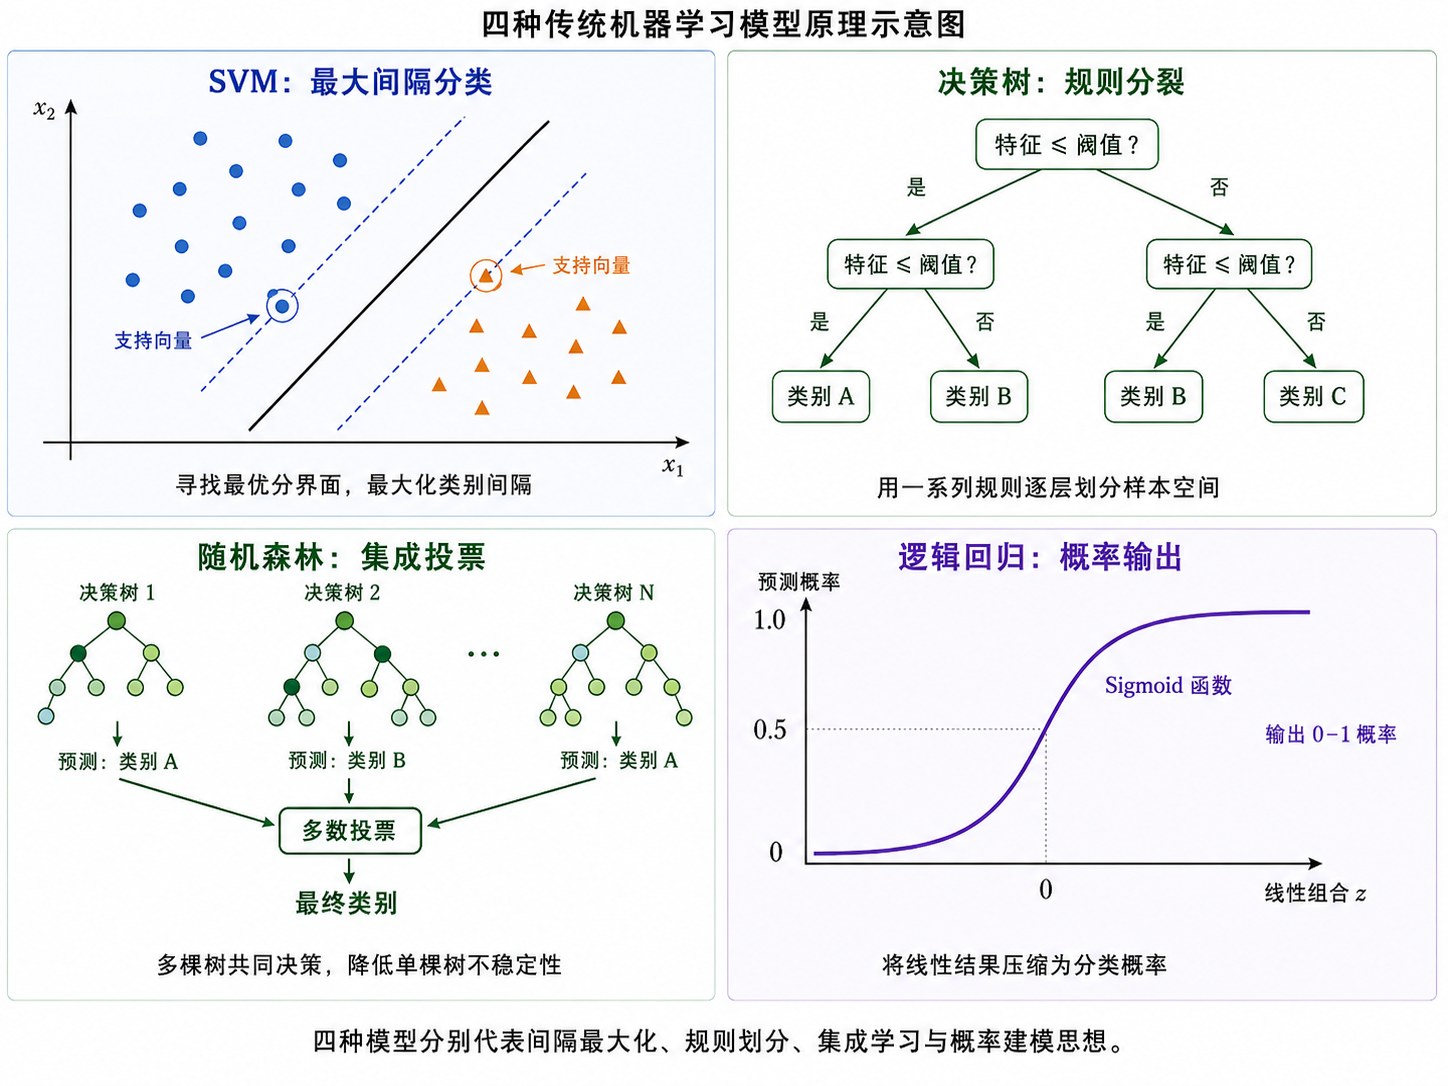
\includegraphics[width=0.92\textwidth]{fig_ml_models.png}
  \caption{四种传统机器学习模型原理示意：间隔最大化、规则分裂、集成投票与概率输出}
  \label{fig:ml-models}
\end{figure}

\subsection{评价指标}
为全面评价模型表现，本文采用准确率、宏平均精确率、宏平均召回率和宏平均 F1 作为基础指标。考虑到类别
分布不均衡和质量等级具有顺序关系，进一步引入平衡准确率、二次加权 Kappa、Cohen's Kappa、MCC 和宏平均
ROC-AUC 等进阶指标。其中，二次加权 Kappa 对跨级误判惩罚更高，适合分析有序标签场景。

准确率表示所有样本中预测正确的比例，适合反映总体分类水平。对类别 $c$ 而言，精确率、召回率和 F1 可写为：
\begin{equation}
P_c=\frac{TP_c}{TP_c+FP_c},\qquad
R_c=\frac{TP_c}{TP_c+FN_c},\qquad
F1_c=\frac{2P_cR_c}{P_c+R_c}.
\end{equation}
宏平均指标对各类别结果直接取平均，使少数类别也能在总体评价中占有相同权重。平衡准确率本质上是各类别召回率
的平均值，能够观察模型是否只偏向样本数较多的类别。MCC 综合考虑混淆矩阵中的四类统计量，在类别不均衡场景下
比单纯准确率更稳定。Cohen's Kappa 衡量预测结果与真实标签的一致性，并扣除随机一致的影响；二次加权 Kappa
进一步按照类别距离设置惩罚权重，因此更适合低、中、高这类有序标签。宏平均 ROC-AUC 则从阈值变化角度评价
模型的类别区分能力，可作为概率输出质量的补充参考。

% ===================== 第三章 数据集与预处理 =====================
\section{数据集与预处理}

\subsection{数据集来源}
本文采用 UCI 机器学习仓库公开的 \href{https://archive.ics.uci.edu/dataset/186/wine+quality}{Wine Quality Data Set}
中的白葡萄酒子集。该子集共 4898 个样本，每个样本包含 11 个理化指标和一个质量评分标签。主要特征包括
固定酸度、挥发性酸度、柠檬酸、残糖、氯化物、游离二氧化硫、总二氧化硫、密度、pH 值、硫酸盐和酒精度。
这些变量均来自理化检测结果，具有明确的物理或化学含义。与人工主观评分相比，理化指标更容易通过仪器稳定
测量，因此适合作为质量分级模型的输入特征。需要注意的是，理化指标能够反映葡萄酒质量的部分侧面，但并不能
完全替代真实品鉴过程中的香气、口感和风格偏好。因此，本文的建模目标更准确地说是基于可观测理化指标对质量
等级进行统计预测，而不是给出完整的感官评价结论。

\subsection{数据查看}
实验首先对数据进行描述性统计、缺失值检查和质量评分分布分析。结果显示，数据集中无缺失值，原始质量
评分主要集中在 5、6、7 三档，极高或极低评分样本较少。图~\ref{fig:quality-dist} 给出了质量评分分布，
图~\ref{fig:corr} 给出了特征相关性热力图。

质量评分分布说明，该数据集存在明显的中间等级集中现象。如果直接预测原始整数评分，部分少数分值的训练样本
不足，容易导致模型对极端评分学习不充分。相关性热力图显示，部分特征之间存在较强相关关系，例如密度与残糖、
酒精度等变量之间具有一定关联。这一现象提示模型需要处理特征间的联合影响，单一变量很难完全解释质量等级。
因此，本文在建模时同时保留全部 11 个理化指标，并通过不同模型比较其非线性组合能力。

\begin{figure}[H]
  \centering
  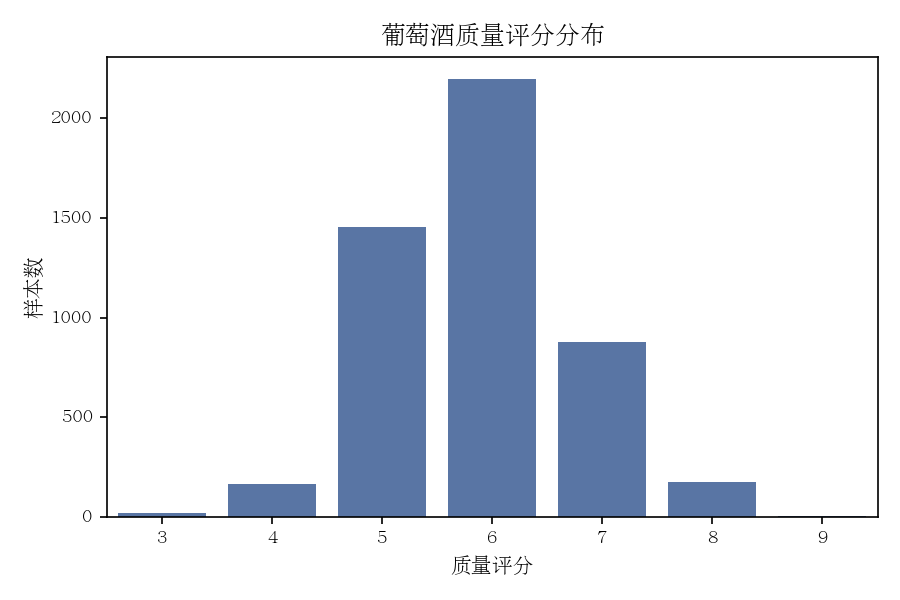
\includegraphics[width=0.58\textwidth]{eda_quality_dist.png}
  \caption{白葡萄酒质量评分分布}
  \label{fig:quality-dist}
\end{figure}

\begin{figure}[H]
  \centering
  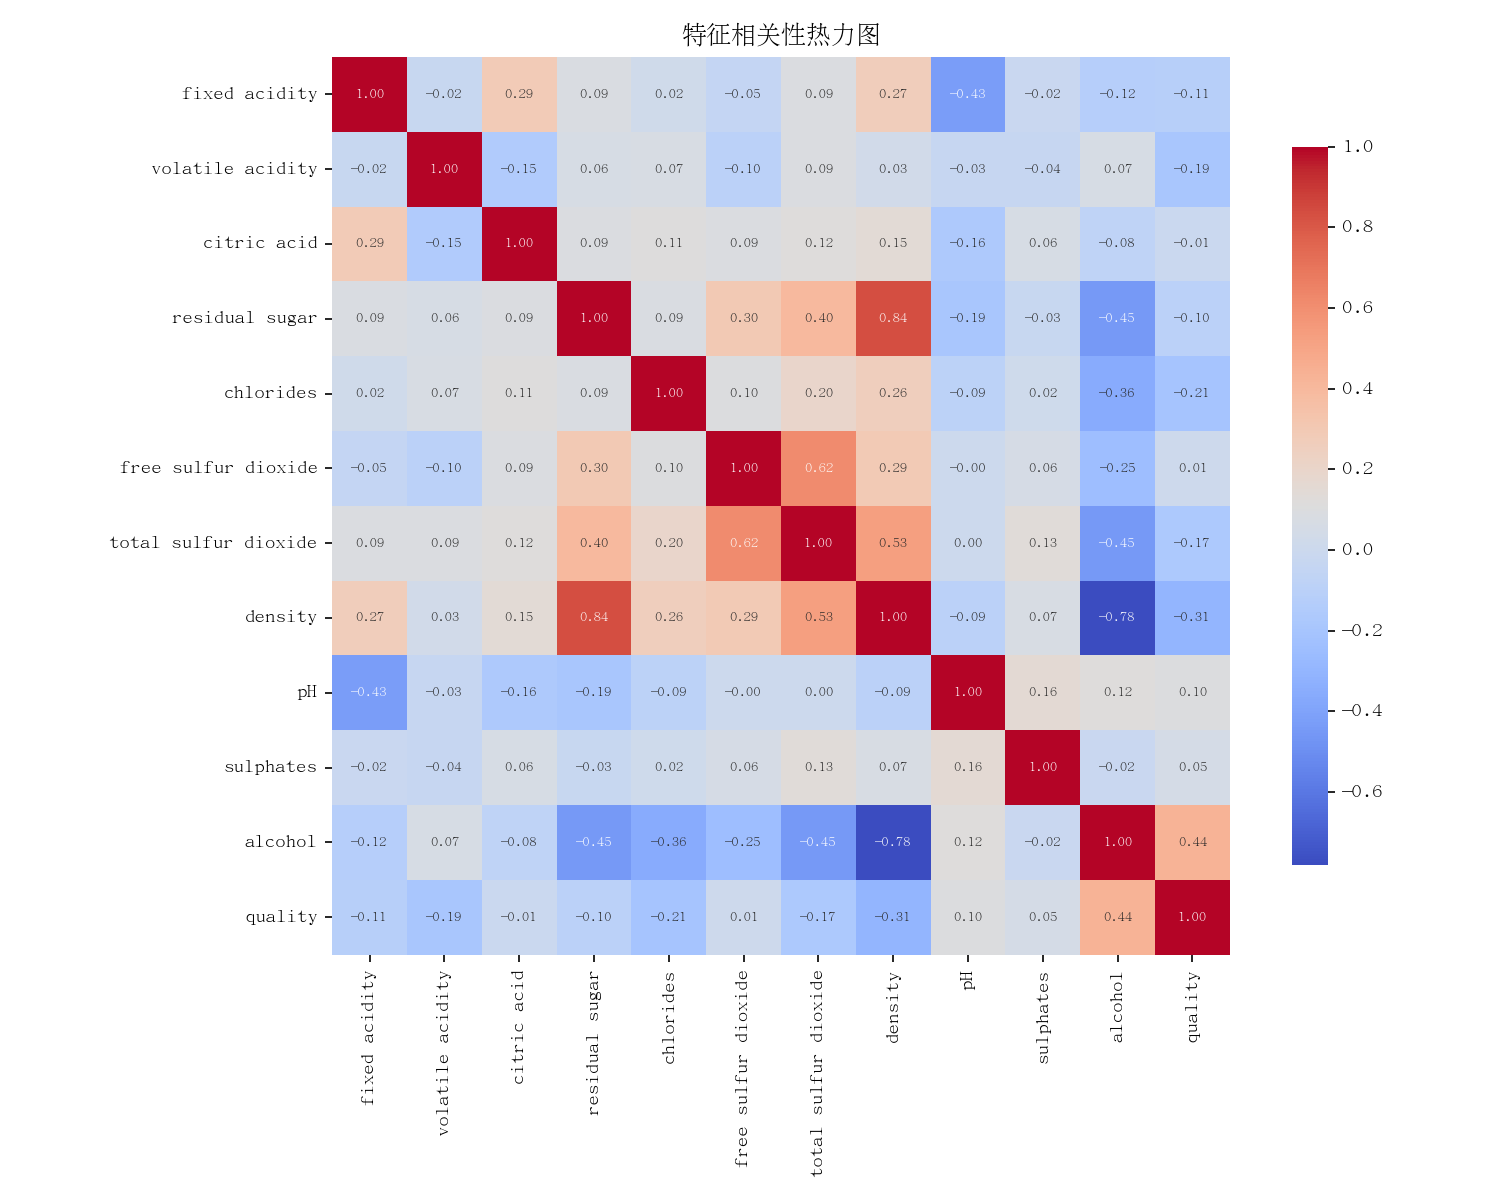
\includegraphics[width=0.8\textwidth]{eda_corr_heatmap.png}
  \caption{理化指标相关性热力图}
  \label{fig:corr}
\end{figure}

\subsection{标签构造与数据划分}
原始质量评分为 0--10 的整数，但实际样本集中主要分布在 5、6、7 分附近。若直接进行多类别分类，少数评分
类别样本过少，模型训练和评价均不稳定。因此，本文结合数据分布与质量分级语义，将评分归并为三类：
\begin{equation}
y=
\begin{cases}
0,&q\le 5,\\
1,&q=6,\\
2,&q\ge 7.
\end{cases}
\end{equation}
其中 0、1、2 分别对应“差”“中”“好”。数据集按 80/20 进行分层划分，保证训练集和测试集中的类别比例基本一致。
标准化操作封装在 scikit-learn 的 \texttt{Pipeline} 中，使 \texttt{StandardScaler} 只在每个训练折内拟合，
避免交叉验证中的数据泄漏。

上述分级方式兼顾了类别可学习性和任务解释性。将 $q\le5$ 归为较低质量，可以覆盖低于主流评分的样本；将
$q=6$ 单独作为中等质量，是因为该分值在数据集中占比较高且处于质量判断的中心区域；将 $q\ge7$ 归为较高质量，
则对应整体表现更好的样本。三分类标签虽然降低了原始评分的细粒度，但能够减少少数类别过稀带来的评估波动，
也更符合实际质量筛选中“较差、一般、较好”的分级需求。分层划分保证测试集中仍保留三类样本的近似比例，
使混淆矩阵和宏平均指标具有可比较性。

% ===================== 第四章 模型建立与实验结果 =====================
\section{模型建立与实验结果}

\subsection{训练设置}
四种模型均采用五折交叉验证和网格搜索进行超参数选择，优化目标为宏平均 F1。各模型搜索空间如表~\ref{tab:grid}
所示。

参数网格的设置遵循“覆盖主要复杂度变化、避免过大搜索成本”的原则。SVM 重点搜索惩罚系数 $C$ 和 RBF 核参数
$\gamma$，前者控制间隔约束与训练误差之间的权衡，后者影响样本相似度的局部性。决策树和随机森林主要搜索树深度、
叶子节点样本数和树数量，以控制过拟合与集成稳定性。逻辑回归搜索正则化强度，用于确定线性基线在不同约束下的
最佳表现。由于本文比较的重点是模型类型和误差结构，而非极限刷分，参数范围保持相对克制，以便结果分析更加清晰。

\begin{figure}[H]
  \centering
  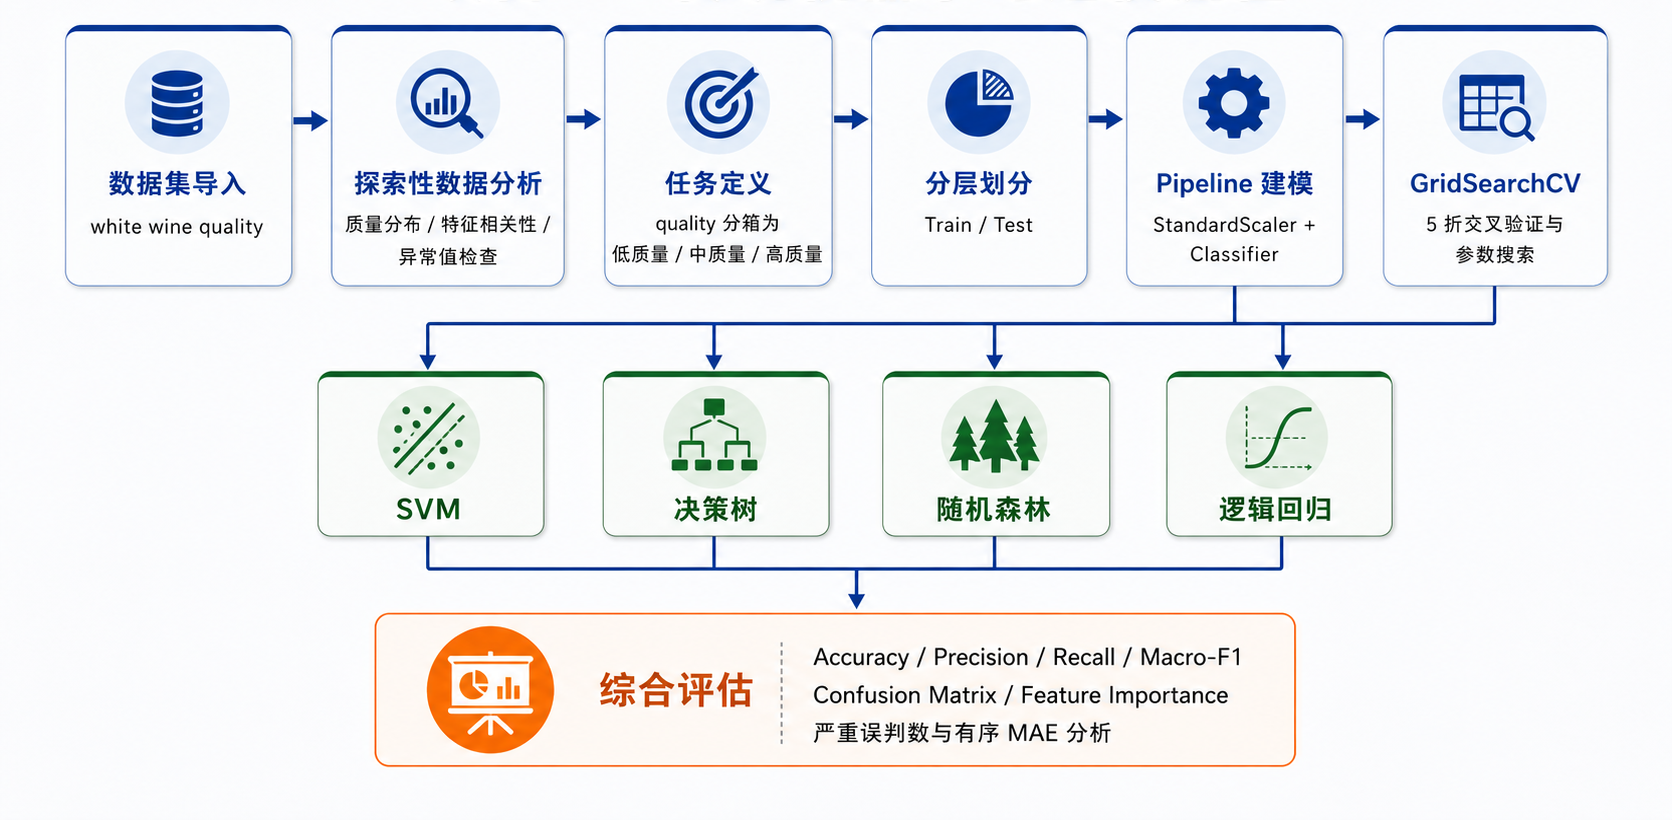
\includegraphics[width=0.95\textwidth]{fig_ml_pipeline.png}
  \caption{任务一传统机器学习建模流程}
  \label{fig:ml-pipeline}
\end{figure}

\begin{table}[H]
  \centering
  \caption{模型超参数搜索空间与最优结果}
  \label{tab:grid}
  \begin{tabular}{lll}
    \toprule
    模型 & 搜索空间 & 最优参数 \\
    \midrule
    SVM & $C\in\{1,10\}$，$\gamma\in\{\mathrm{scale},0.1\}$ & $C=10$，$\gamma=0.1$ \\
    决策树 & 最大深度 $\in\{\mathrm{None},10,20\}$，叶子样本 $\in\{1,5\}$ & 深度 None，叶子样本 1 \\
    随机森林 & 树数 $\in\{200,400\}$，最大深度 $\in\{\mathrm{None},20\}$ & 树数 200，深度 20 \\
    逻辑回归 & $C\in\{0.5,1,10\}$ & $C=0.5$ \\
    \bottomrule
  \end{tabular}
\end{table}

\subsection{基础指标结果}
四种模型在测试集上的基础指标如表~\ref{tab:metric} 所示。随机森林在准确率、精确率、召回率和宏平均 F1 上
均取得较好结果，说明集成学习能够较好拟合理化指标与质量等级之间的非线性关系。

\begin{table}[H]
  \centering
  \caption{四种模型的基础评估指标（测试集）}
  \label{tab:metric}
  \begin{tabular}{lcccc}
    \toprule
    模型 & 准确率 & 精确率 & 召回率 & 宏平均 F1 \\
    \midrule
    SVM & 0.617 & 0.616 & 0.660 & 0.622 \\
    决策树 & 0.650 & 0.647 & 0.644 & 0.645 \\
    \textbf{随机森林} & \textbf{0.735} & \textbf{0.748} & \textbf{0.723} & \textbf{0.734} \\
    逻辑回归 & 0.522 & 0.524 & 0.567 & 0.520 \\
    \bottomrule
  \end{tabular}
\end{table}

\begin{figure}[H]
  \centering
  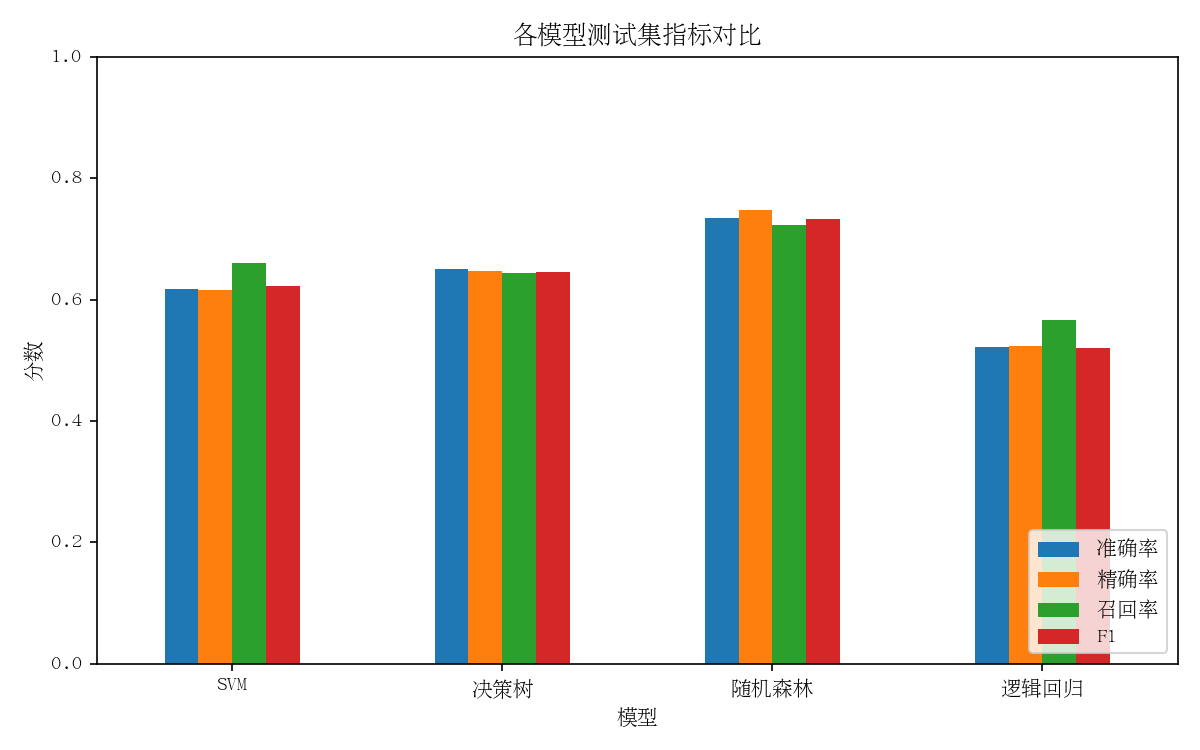
\includegraphics[width=0.78\textwidth]{model_compare.png}
  \caption{四种模型测试集指标对比}
  \label{fig:model-compare}
\end{figure}

从模型对比看，逻辑回归的准确率和宏平均 F1 均最低，说明理化指标与三类质量标签之间并非简单线性可分。SVM
借助 RBF 核能够表达非线性边界，但在本实验中整体性能仍低于树模型，可能与质量等级边界模糊、特征间存在复杂
交互以及类别分布不均衡有关。单棵决策树相比逻辑回归和 SVM 有一定提升，但其划分规则受局部样本影响较大，
泛化稳定性有限。随机森林通过多棵树集成缓解了单树方差问题，在四项基础指标上均取得最高值，说明其更适合
处理该数据集中理化指标之间的非线性组合关系。

同时，随机森林准确率为 0.7347，宏平均 F1 为 0.7336，两者较为接近，说明模型并非仅依赖某个多数类别获得
较高准确率，而是在三个类别上保持了相对均衡的识别能力。不过，该结果也表明任务本身仍有明显难度：质量评分
受到感官主观性和潜在未观测因素影响，仅依赖 11 个理化指标难以完全区分所有边界样本。因此，后续分析需要结合
混淆矩阵和有序误差，而不能只依据总体准确率判断模型表现。

\subsection{进阶指标结果}
表~\ref{tab:extra} 给出了进阶评估指标。随机森林在平衡准确率、二次加权 Kappa、MCC 和宏平均 ROC-AUC 等指标上
也取得最高结果，说明其优势不仅体现在总体准确率上，也体现在有序一致性和不平衡鲁棒性等方面。

\begin{table}[H]
  \centering
  \caption{四种模型的进阶评估指标（测试集）}
  \label{tab:extra}
  \resizebox{\textwidth}{!}{%
  \begin{tabular}{lccccc}
    \toprule
    模型 & 平衡准确率 & 二次加权 Kappa & Cohen's Kappa & MCC & 宏 ROC-AUC \\
    \midrule
    SVM & 0.660 & 0.626 & 0.428 & 0.439 & 0.819 \\
    决策树 & 0.644 & 0.566 & 0.451 & 0.452 & 0.729 \\
    \textbf{随机森林} & \textbf{0.723} & \textbf{0.720} & \textbf{0.579} & \textbf{0.581} & \textbf{0.899} \\
    逻辑回归 & 0.567 & 0.491 & 0.296 & 0.311 & 0.740 \\
    \bottomrule
  \end{tabular}}
\end{table}

平衡准确率结果进一步说明，随机森林对不同类别的召回能力较为均衡。二次加权 Kappa 达到 0.720，表示预测结果
与真实等级之间具有较好的一致性，并且严重跨级误判相对较少。MCC 为 0.581，说明模型预测与真实标签之间存在
较稳定的相关关系，但仍未达到完全可靠的程度。宏平均 ROC-AUC 为 0.899，说明随机森林输出的类别概率具有较好
排序能力，即使某些样本最终类别判断错误，模型仍能在概率层面对类别进行相对有效的区分。相比之下，决策树的
ROC-AUC 仅为 0.729，提示单树概率估计和边界稳定性均较弱。

\subsection{随机森林模型分析}
随机森林各类别指标如表~\ref{tab:rf-class} 所示。模型对“差”和“好”两端类别的精确率较高，而“中”类样本
与相邻等级边界较模糊，分类难度相对更高。

\begin{table}[H]
  \centering
  \caption{随机森林各类别精确率、召回率和 F1}
  \label{tab:rf-class}
  \begin{tabular}{lcccc}
    \toprule
    类别 & 精确率 & 召回率 & F1 & 样本数 \\
    \midrule
    差（$\le 5$） & 0.78 & 0.73 & 0.76 & 328 \\
    中（$=6$） & 0.69 & 0.77 & 0.73 & 440 \\
    好（$\ge 7$） & 0.77 & 0.67 & 0.72 & 212 \\
    \bottomrule
  \end{tabular}
\end{table}

\begin{figure}[H]
  \centering
  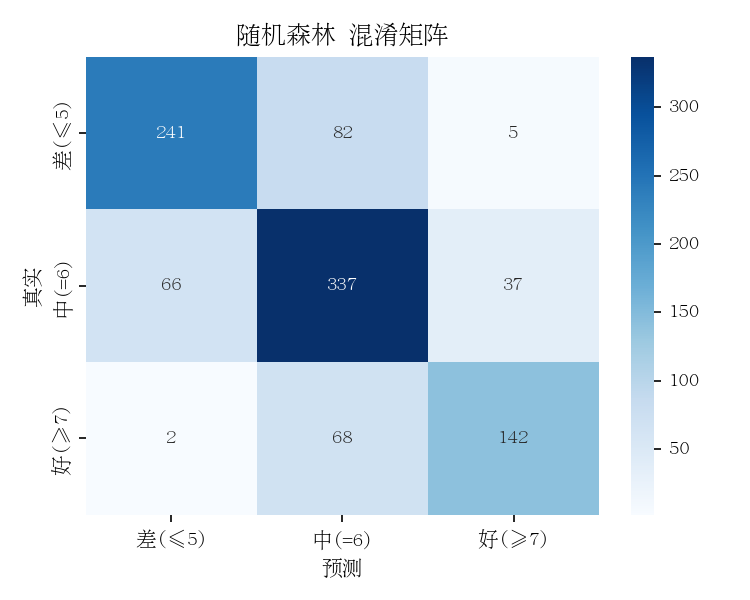
\includegraphics[width=0.55\textwidth]{cm_random_forest.png}
  \caption{随机森林混淆矩阵}
  \label{fig:rf-cm}
\end{figure}

随机森林的特征重要性如图~\ref{fig:rf-imp} 所示。酒精度、密度和挥发性酸度对质量等级判别贡献较大，这与
相关性分析结果基本一致。

从各类别指标看，“差”类 F1 为 0.76，“中”类 F1 为 0.73，“好”类 F1 为 0.72，三类之间差距不大，但召回率
分布存在差异。中等质量样本召回率较高，说明模型较容易将边界不明确的样本归入中间等级；较高质量样本召回率
相对偏低，说明部分高质量样本会被预测为中等质量。这种现象与数据分布和评分语义一致：中间等级样本数量更多，
且很多理化指标处于连续变化状态，导致“中”和“好”之间不存在清晰的硬边界。

\begin{figure}[H]
  \centering
  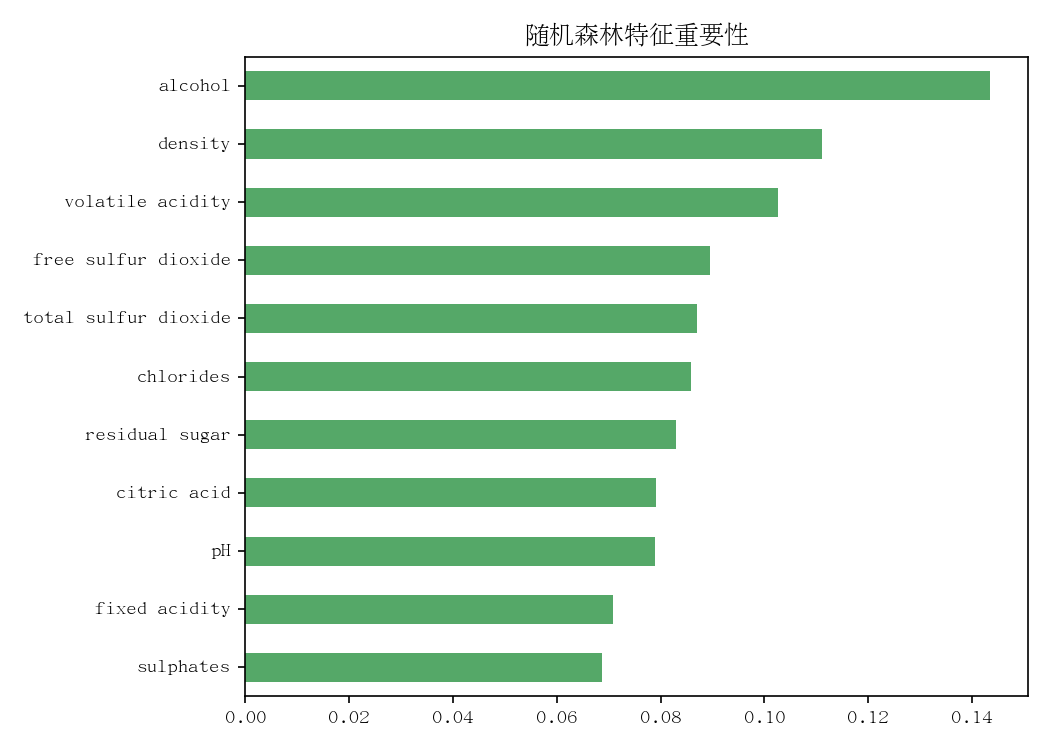
\includegraphics[width=0.7\textwidth]{rf_feature_importance.png}
  \caption{随机森林特征重要性排序}
  \label{fig:rf-imp}
\end{figure}

特征重要性排序可作为模型解释的参考，但不应被理解为严格因果关系。酒精度较高的重要性说明其在树模型划分中
经常提供有效信息；密度与残糖、酒精度等变量存在关联，因此在区分不同质量等级时也可能发挥作用；挥发性酸度
通常与不良风味相关，其重要性较高也符合葡萄酒质量判断的常识。由于随机森林重要性会受到特征相关性的影响，
当多个变量携带相近信息时，重要性可能在相关特征之间分散。因此，本文将其作为解释模型判别依据的辅助结果，
而不是对理化机制作绝对判断。

% ===================== 第五章 误差分析与补充实验 =====================
\section{误差分析与补充实验}

\subsection{邻级混淆现象}
进一步分析随机森林混淆矩阵可以发现，模型错误主要集中于“差”和“中”、“中”和“好”之间，而“差”和“好”
之间的严重跨级误判较少。这说明质量等级边界具有模糊性，模型较难区分相邻等级，但整体上能够保持较好的
有序一致性。

这种邻级混淆具有明确的任务含义。对于葡萄酒质量评分而言，从 5 分到 6 分、从 6 分到 7 分的差异往往对应
若干理化指标和感官因素的综合变化，边界样本在特征空间中可能相互重叠。相较之下，将低质量样本误判为高质量
或将高质量样本误判为低质量，会带来更大的业务风险。随机森林严重跨级误判较少，说明模型虽然无法完全解决
相邻等级边界问题，但在质量等级的整体排序方向上具有一定稳定性。也正因为如此，单纯三分类准确率不足以完整
描述模型价值，有必要引入有序评价指标和补充实验。

\subsection{有序回归分级对照}
由于葡萄酒质量评分具有天然顺序，本文补充采用“回归预测连续质量分，再按阈值分级”的方式进行对照。评价
指标除准确率和宏平均 F1 外，还引入严重误判数和有序 MAE。结果如表~\ref{tab:ordinal} 和图~\ref{fig:ordinal}
所示。

\begin{table}[H]
  \centering
  \caption{直接分类与有序回归分级的对比}
  \label{tab:ordinal}
  \resizebox{\textwidth}{!}{%
  \begin{tabular}{lccccc}
    \toprule
    方法 & 准确率 & 宏平均 F1 & 二次加权 Kappa & 严重误判数 & 有序 MAE \\
    \midrule
    直接分类（随机森林） & 0.7347 & 0.7336 & 0.7200 & 7 & 0.2724 \\
    \textbf{有序回归→分级} & \textbf{0.7571} & \textbf{0.7533} & \textbf{0.7411} & \textbf{4} & \textbf{0.2469} \\
    \bottomrule
  \end{tabular}}
\end{table}

\begin{figure}[H]
  \centering
  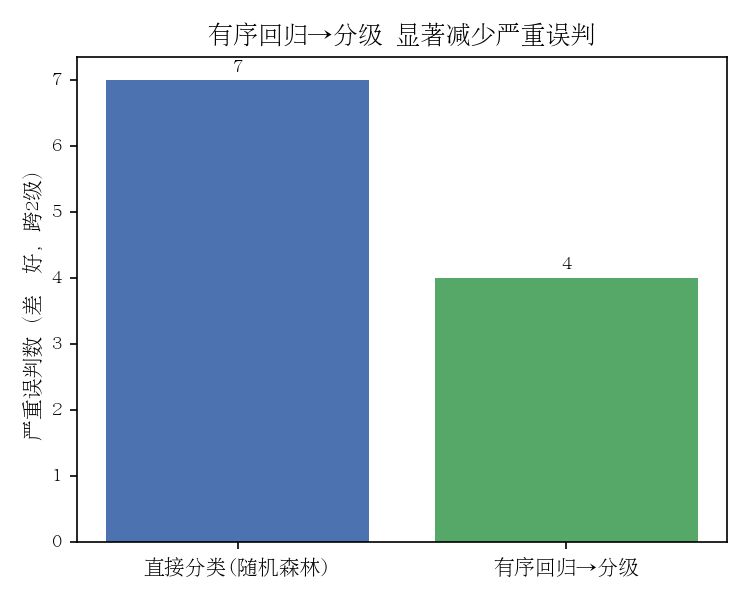
\includegraphics[width=0.52\textwidth]{ordinal_improvement.png}
  \caption{有序回归分级减少严重误判}
  \label{fig:ordinal}
\end{figure}

结果显示，有序回归分级在多项指标上取得提升，尤其是严重跨级误判数由 7 降至 4。这说明在质量等级具有
自然顺序的场景中，将标签有序性纳入建模和评价过程具有实际意义。

有序回归分级的改进并不意味着常规分类方法失效，而是说明该任务中“类别距离”包含了有用信息。直接分类把
“差、中、好”视为三个相互独立的标签，模型优化时不会显式区分相邻误判和跨级误判；回归再分级则先预测连续
质量分，再根据阈值映射到等级，因此天然保留了评分从低到高的顺序结构。其准确率由 0.7347 提升至 0.7571，
宏平均 F1 由 0.7336 提升至 0.7533，有序 MAE 也有所下降，说明该策略对边界样本具有一定缓和作用。
不过，该对照仍属于较基础的有序建模尝试，结论应限定在当前数据划分和模型配置下。若要进一步确认稳定性，
还需要多随机种子重复实验，并比较专门的有序分类模型。

% ===================== 第六章 跨数据集模型对照研究 =====================
\section{跨数据集模型对照研究}

前述各章均围绕白葡萄酒一个数据集展开。为进一步回答“究竟是什么决定了传统机器学习模型的分类性能”这一
问题，本章\textbf{以四种模型本身为研究对象}，把同一套建模管线推广到难度递增的五个结构化数据集上对照，
考察模型表现如何随数据特点变化。本章核心结论是：\textbf{不存在放之四海而皆准的“最优模型”，性能由数据
特点与“模型—数据匹配”共同决定}。

\subsection{实验设置：难度阶梯与统一模型管线}
本章在白葡萄酒之外，另选取四个公开结构化数据集：电离层雷达回波（ionosphere）、贷款违约预测
（Lending Club）、干豆形态分类（Dry Bean）和臭氧层超标检测（Ozone）。五个数据集在样本量、特征维度、
类别数和类别平衡程度上差异明显，构成由易到难的难度阶梯，其基本特征如表~\ref{tab:tab-ds} 所示。其中
Lending Club 原始数据约 1.19\,GB，本文仅取已结清贷款（Fully Paid/Charged Off）、剔除回款额等会泄露
标签的事后特征，并按类别分层抽样 3 万条以保证可计算性。

\begin{table}[H]
  \centering
  \caption{五个结构化数据集的基本特征}
  \label{tab:tab-ds}
  \resizebox{\textwidth}{!}{%
  \begin{tabular}{lccccl}
    \toprule
    数据集 & 样本数 & 特征维度 & 类别数 & 不平衡比 & 特点 \\
    \midrule
    电离层 ionosphere & 351 & 34 & 2 & 1.8 & 小样本、近线性可分 \\
    白葡萄酒 wine & 4898 & 11 & 3 & 2.1 & 有序、轻度不平衡 \\
    贷款违约 Lending Club & 30000 & 12 & 2 & 4.0 & 大规模、弱信号 \\
    干豆 Dry Bean & 13611 & 16 & 7 & 6.8 & 多分类、形态可分 \\
    臭氧 Ozone & 2536 & 72 & 2 & 33.7 & 高维、极度不平衡 \\
    \bottomrule
  \end{tabular}}
\end{table}

五个数据集由易到难的难度阶梯及其关键特征如图~\ref{fig:tab-datasets} 所示。

\begin{figure}[H]
  \centering
  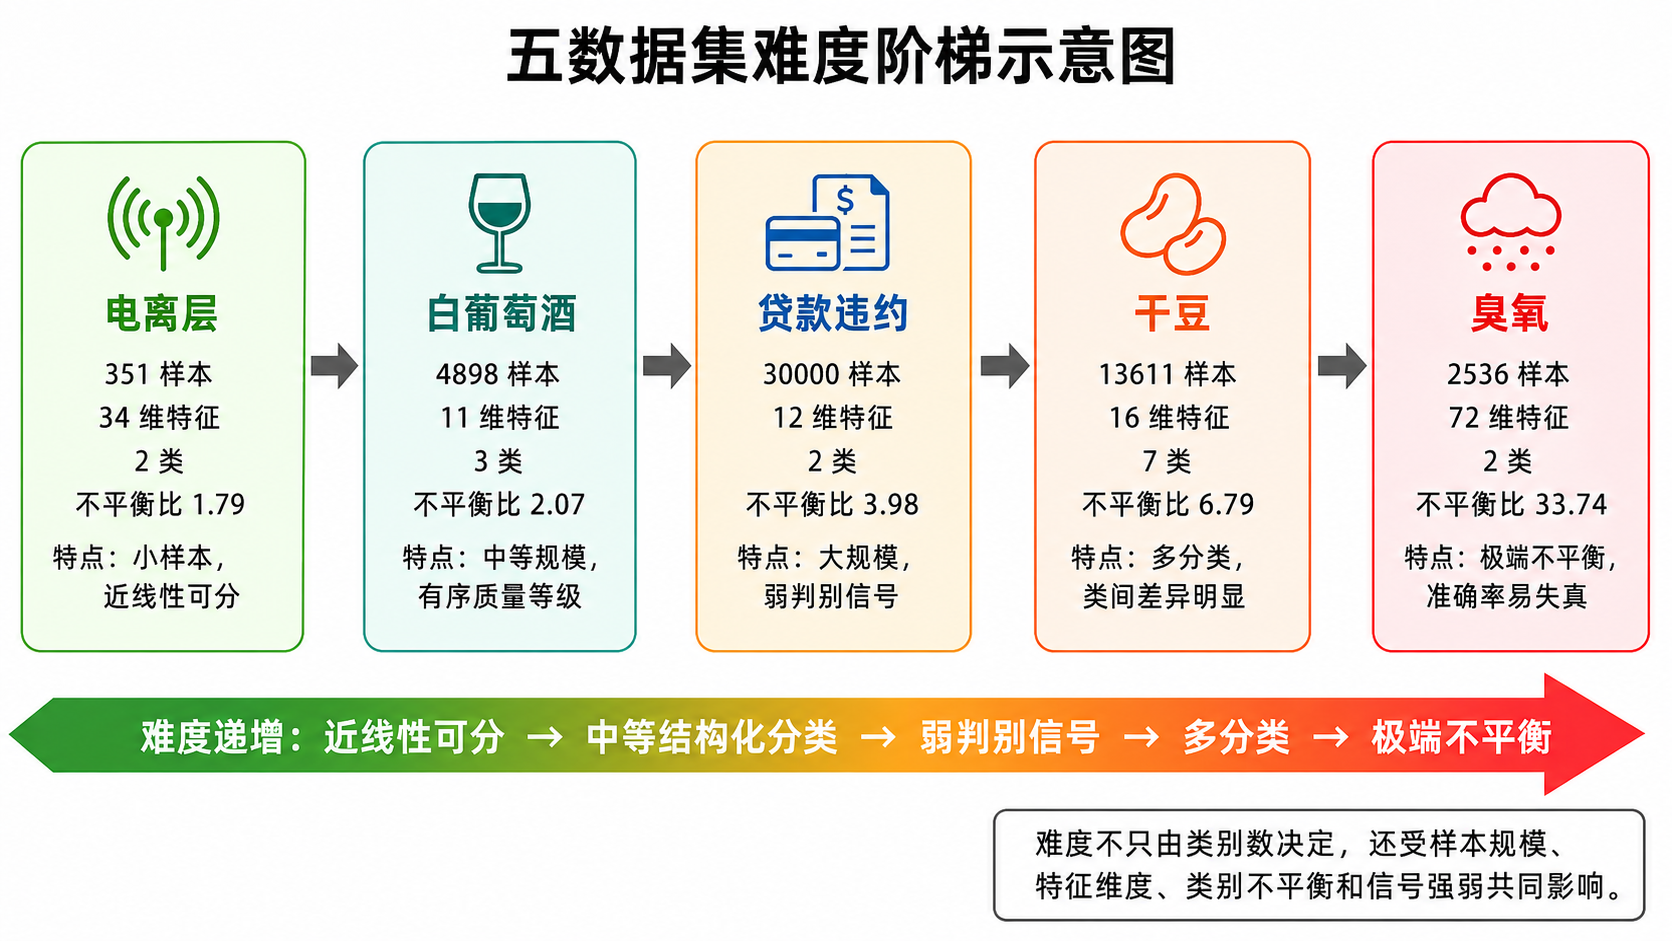
\includegraphics[width=0.95\textwidth]{fig_tab_datasets.png}
  \caption{五个结构化数据集的难度阶梯：从小样本近线性可分到大规模弱信号、多分类与极端不平衡}
  \label{fig:tab-datasets}
\end{figure}

为保证对照公平，五个数据集统一采用相同的建模管线：标准化、五折交叉验证和网格搜索，并对每个数据集使用
完全相同的四种模型（SVM、决策树、随机森林、逻辑回归）及其超参数搜索空间，评价主指标为宏平均 F1，
辅以准确率与平衡准确率。所有模型均开启类别权重平衡（class\_weight=balanced）。

\subsection{跨数据集对照结果}
四种模型在五个数据集上的测试集宏平均 F1 如表~\ref{tab:tab-f1} 和图~\ref{fig:tab-f1} 所示。可以看到，
\textbf{最优模型随数据集而改变}：随机森林在电离层和白葡萄酒上最好，支持向量机在干豆上最好，逻辑回归在
贷款违约上最好，而在极不平衡的臭氧上各模型表现都很差。这直观印证了“没有免费午餐”——没有任何单一模型
在所有任务上占优。

\begin{table}[H]
  \centering
  \caption{四种模型在五个数据集上的测试集宏平均 F1}
  \label{tab:tab-f1}
  \resizebox{\textwidth}{!}{%
  \begin{tabular}{lccccc}
    \toprule
    数据集 & SVM & 决策树 & 随机森林 & 逻辑回归 & 最优模型 \\
    \midrule
    电离层 ionosphere & 0.9393 & 0.9235 & \textbf{0.9541} & 0.8598 & 随机森林 \\
    白葡萄酒 wine & 0.6219 & 0.6449 & \textbf{0.7336} & 0.5204 & 随机森林 \\
    贷款违约 Lending Club & 0.5698 & 0.5379 & 0.5275 & \textbf{0.5843} & 逻辑回归 \\
    干豆 Dry Bean & \textbf{0.9375} & 0.9104 & 0.9333 & 0.9300 & SVM \\
    臭氧 Ozone & \textbf{0.5805} & 0.5653 & 0.4920 & 0.5704 & SVM \\
    \bottomrule
  \end{tabular}}
\end{table}

\begin{figure}[H]
  \centering
  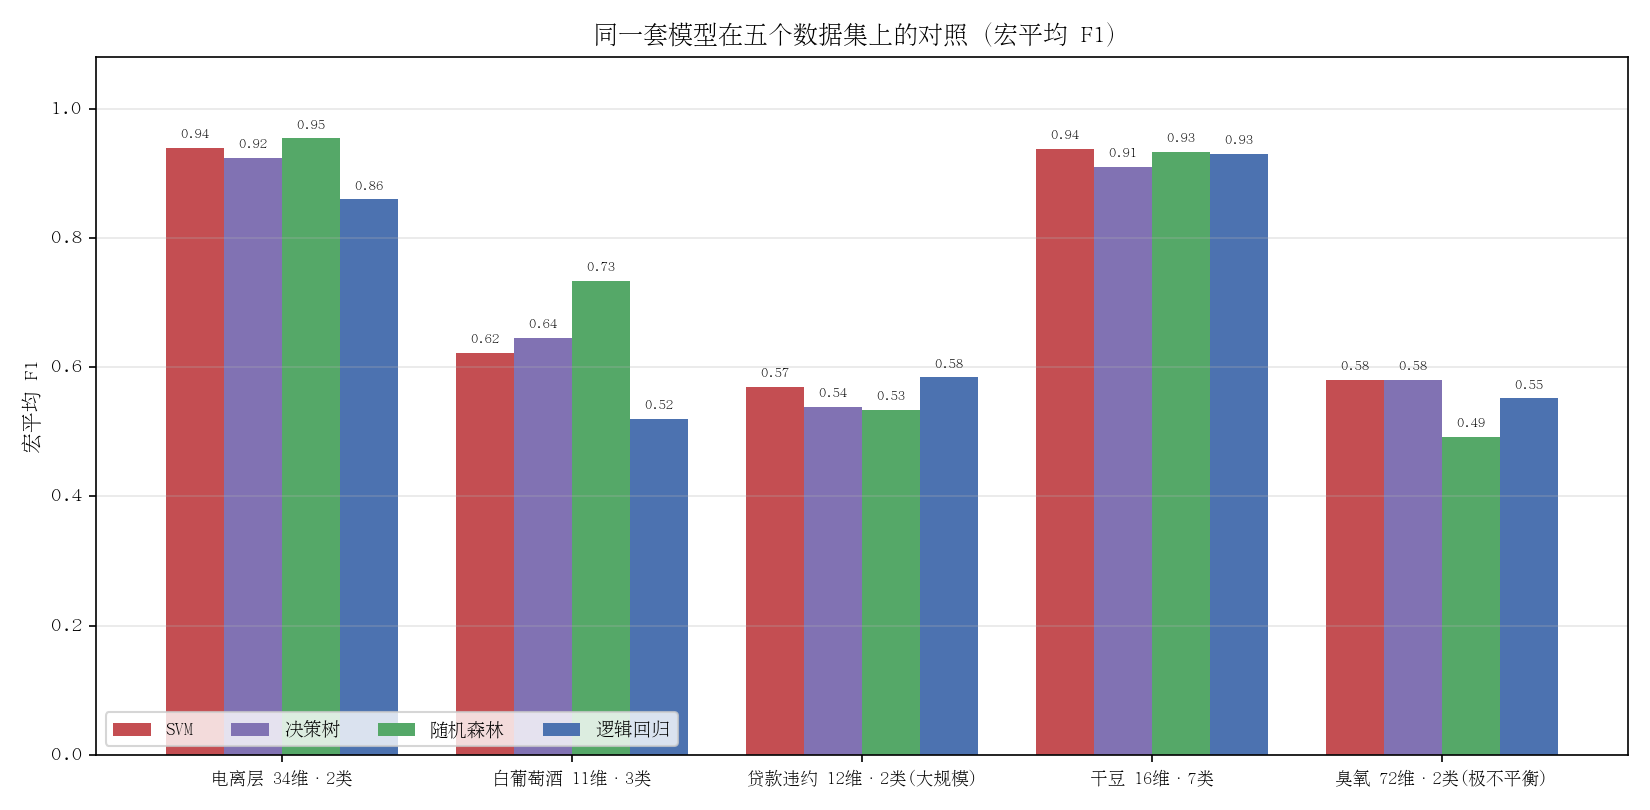
\includegraphics[width=0.95\textwidth]{cross_tab_f1.png}
  \caption{同一套模型在五个数据集上的宏平均 F1 对照}
  \label{fig:tab-f1}
\end{figure}

从结果可归纳出几点规律。其一，在特征干净、类别较可分的数据集上（电离层、干豆），四种模型差距不大、
整体都较高，说明此时数据本身的可分性决定了上限，模型选择影响有限；值得注意的是干豆虽有 7 个类别，
各模型宏平均 F1 仍达 0.91 以上，说明\textbf{类别数量并非决定难度的主要因素}，这与项目二的结论一致。
其二，随机森林在中低维、非线性、较平衡的数据上通常是稳健的默认选择（白葡萄酒上以 0.7336 显著领先）。
其三，逻辑回归在近线性可分或弱信号数据上反而更稳（贷款违约上最优），说明当特征与标签关系接近线性、
或信号本身较弱时，复杂模型并无优势。

\subsection{不平衡与“本质困难”：准确率的陷阱}
跨数据集对照还暴露了两类容易被准确率掩盖的问题，如图~\ref{fig:tab-imb} 所示。极端不平衡下“准确率虚高、
实则失效”的机理如图~\ref{fig:imb-trap} 所示。

\begin{figure}[H]
  \centering
  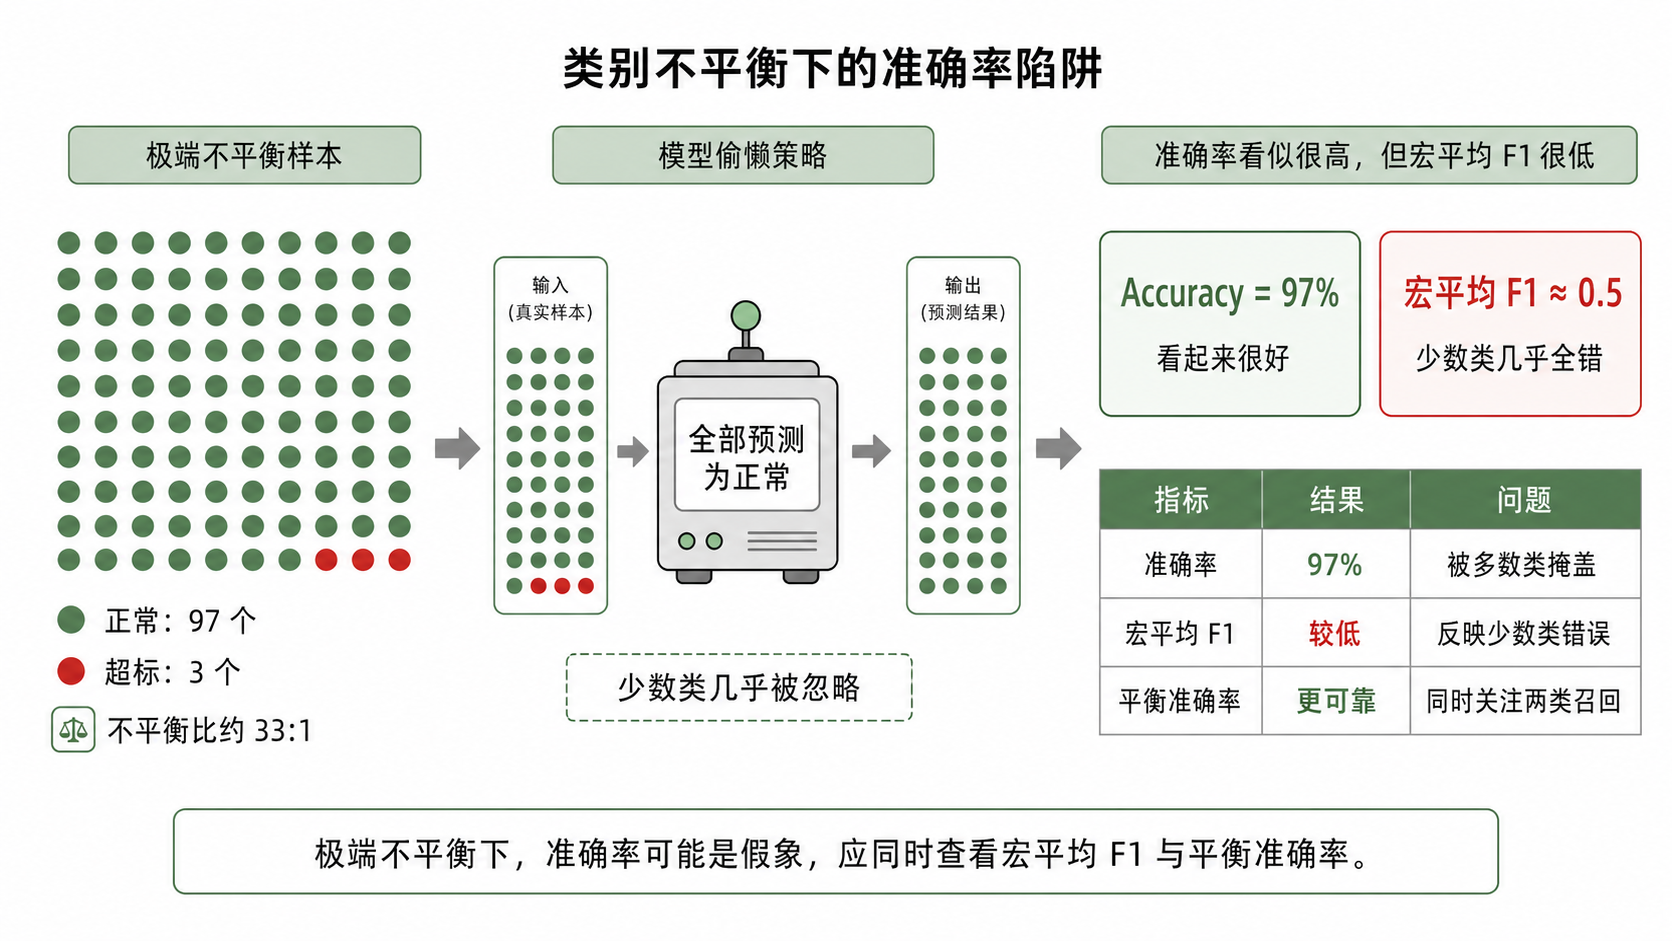
\includegraphics[width=0.95\textwidth]{fig_imbalance_trap.png}
  \caption{类别不平衡下的准确率陷阱：33:1 时“全预测多数类”即得 97\% 准确率，但宏 F1 仅约 0.5}
  \label{fig:imb-trap}
\end{figure}

\begin{figure}[H]
  \centering
  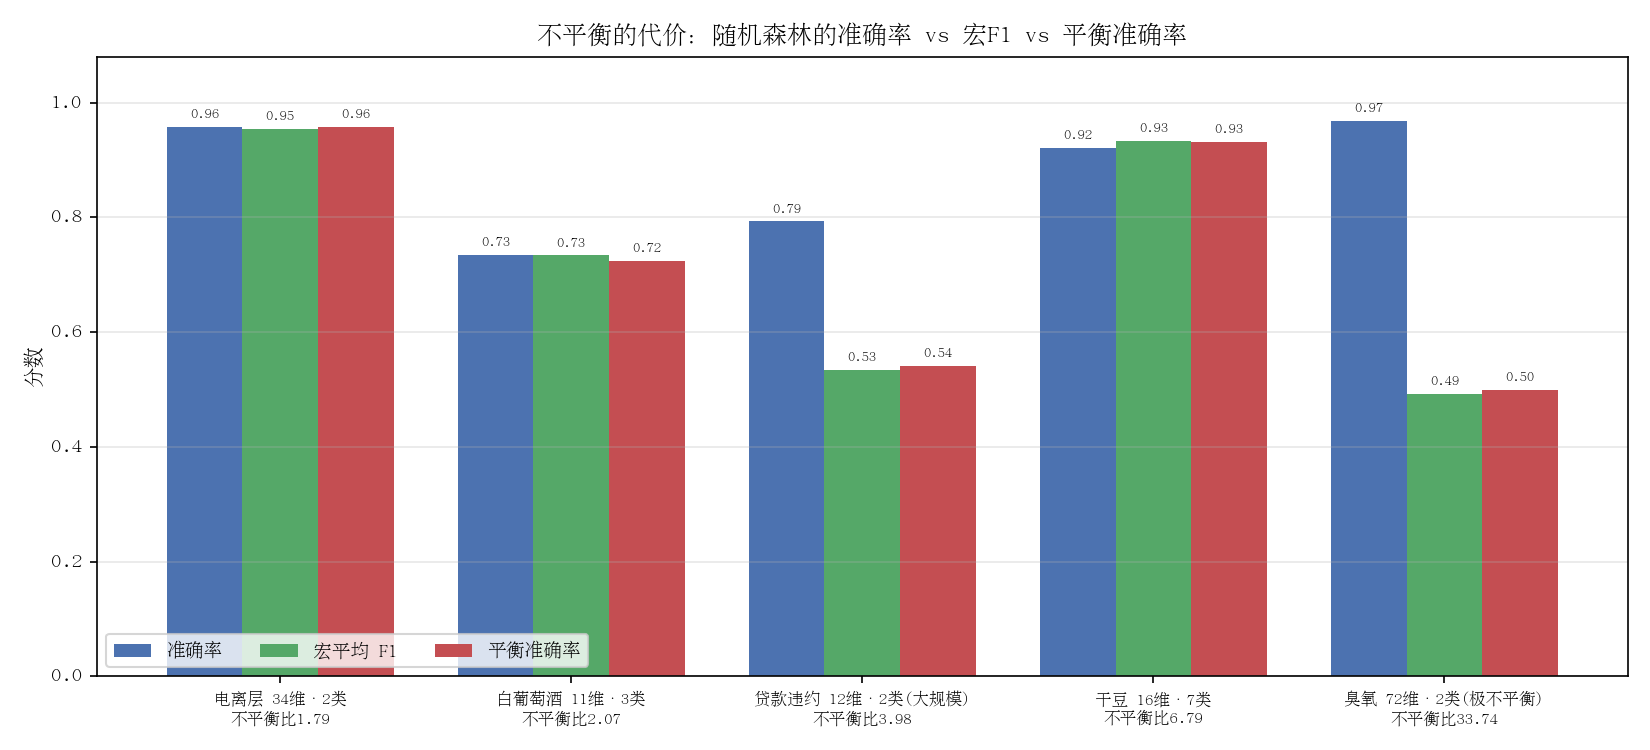
\includegraphics[width=0.95\textwidth]{cross_tab_imbalance.png}
  \caption{不平衡的代价：随机森林的准确率、宏平均 F1 与平衡准确率对照}
  \label{fig:tab-imb}
\end{figure}

第一类是\textbf{极端类别不平衡}。臭氧数据集阳性样本仅占 2.9\%，不平衡比高达 33.7。此时“全部预测为多数
类”即可得到 97.05\% 的准确率；随机森林测试准确率为 96.85\%，看似很高，却\textbf{反而低于这一多数类
基线}，其宏平均 F1 仅 0.492、平衡准确率仅 0.499（约等于随机猜测）。这说明在极端不平衡下，准确率几乎
没有意义，必须以宏平均 F1 或平衡准确率衡量，否则会得出“模型很好”的错误结论。

第二类是\textbf{数据本身的“本质困难”}。贷款违约预测中，四种模型的宏平均 F1 全部落在 0.53\,$\sim$\,0.58
的狭窄区间，无论选用何种模型都无法显著突破。这是因为可在申请时获得的数值特征对“是否违约”的判别信号
本就较弱，性能瓶颈在数据而非模型——这与项目二“当模型足够强时瓶颈转向数据”的结论相互呼应。

\subsection{针对欠佳数据集的改进尝试与归因}
对于表现欠佳的贷款违约和臭氧两个数据集，本文进一步尝试有针对性的处理，以判断其“效果不好”究竟源于
处理不充分还是数据本质，结果如表~\ref{tab:improve-tab} 所示。

\begin{table}[H]
  \centering
  \caption{两个欠佳数据集的改进尝试（测试集宏平均 F1，取四模型/GBDT 中最优）}
  \label{tab:improve-tab}
  \resizebox{\textwidth}{!}{%
  \begin{tabular}{llcl}
    \toprule
    数据集 & 处理手段 & 最优宏 F1 & 结果与归因 \\
    \midrule
    \multirow{3}{*}{贷款违约}
      & 基线（12 维数值特征） & 0.5843 & --- \\
      & 补充申请时类别特征（37 维） & 0.5902 & 几乎无提升：int\_rate 已编码 grade，信息冗余 \\
      & 梯度提升 GBDT（37 维） & 0.5759 & 更强模型亦无突破 \\
    \midrule
    \multirow{3}{*}{臭氧}
      & 基线（class\_weight 平衡） & 0.5805 & --- \\
      & SMOTE 过采样 & 0.5644 & 不升反降：高维且少数类样本过少，插值成噪声 \\
      & 梯度提升 GBDT & 0.5836 & 仅与基线持平，未突破 \\
    \bottomrule
  \end{tabular}}
\end{table}

\begin{figure}[H]
  \centering
  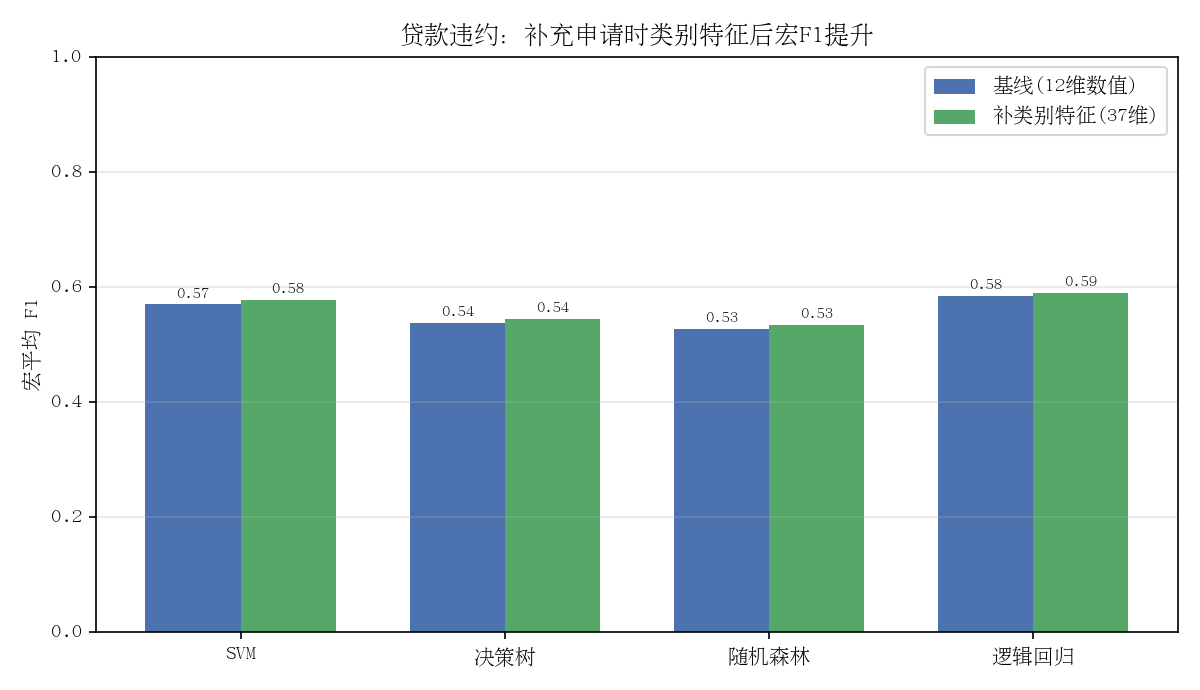
\includegraphics[width=0.78\textwidth]{improve_lendingclub.png}
  \caption{贷款违约：补充申请时类别特征前后的宏平均 F1（几乎持平）}
  \label{fig:improve-lc}
\end{figure}

\begin{figure}[H]
  \centering
  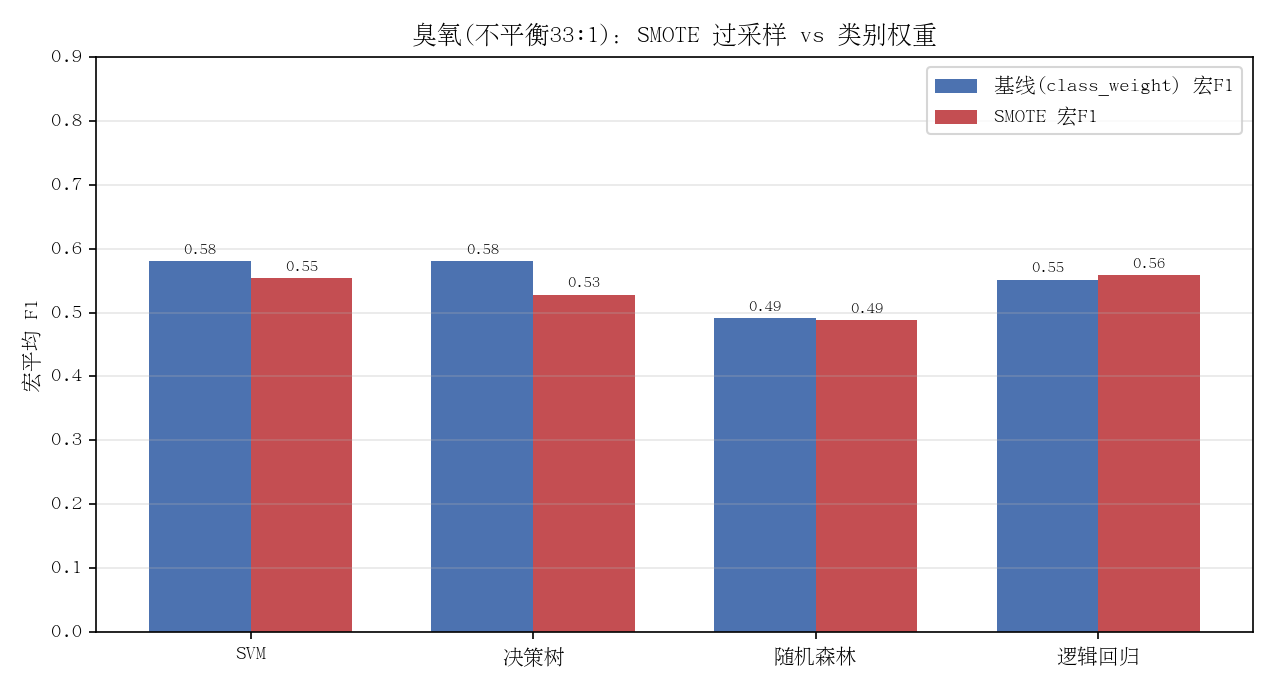
\includegraphics[width=0.80\textwidth]{improve_ozone.png}
  \caption{臭氧：SMOTE 过采样与类别权重的宏平均 F1 对照（SMOTE 未带来改进）}
  \label{fig:improve-oz}
\end{figure}

三种处理手段的结果给出一致结论。其一，为贷款违约补充 grade、期限、工龄等申请时类别特征后，宏平均 F1
几乎不变（0.5843 至 0.5902）。原因在于基线已包含的利率（int\_rate）实际上已经编码了贷款等级——经核验，
A 至 G 级的平均利率由 7.3\% 单调升至 30.8\%，新增的等级特征与之高度共线、信息冗余；而最强的 FICO 信用分
在本数据集版本中并不提供。其二，对极端不平衡（33:1）的臭氧采用 SMOTE 过采样后宏平均 F1 反而下降，
因为该数据集特征高达 72 维而少数类训练样本仅数十个，SMOTE 在高维空间靠极少邻居插值，合成的多为噪声
而非有效样本。其三，进一步换用更强的梯度提升模型（GBDT），两个数据集的宏平均 F1 仍分别停在 0.576 和
0.584，均在约 0.58 的水平，相对四个基础模型未带来稳定提升。

由此可以判断：在当前特征集合、划分方式与参数搜索范围内，补特征、重采样、换更强模型三类手段均未给这两个
数据集带来稳定提升，\textbf{表明其“效果不好”更可能源于弱判别信号或极端不平衡叠加高维小样本等数据本质，
而非单一处理手段的缺失}（需多随机种子进一步确认）。相对而言更有效的是“模型与数据的匹配”：在臭氧上避开
会崩溃的随机森林、改用决策树或支持向量机并配合类别权重，已是该任务的较优选择。
这一“诊断—多手段尝试—归因”的过程，与项目二中“激进数据增强反而有害”的结论相互呼应，都说明改进必须
先判断瓶颈来源，再对症下药。

\subsection{任务级方法创新尝试与严谨评估的教训}
前一节的补特征、重采样、换更强模型属于\textbf{通用静态手段}。为进一步逼问“效果不好”究竟是\emph{建模方式}
没贴合任务结构、还是\emph{数据信息}已到上限，本节针对两个欠佳数据集各设计一项\textbf{任务级方法创新}。其中
臭氧实验还意外给出一条关于\textbf{评估严谨性}的重要教训。

\textbf{（一）臭氧：把“无序表格”还原为“时间序列”。} 经核查，臭氧数据集首列即为采集日期，覆盖
1998—2004 年逐日观测，而基线直接丢弃日期列、随机划分训练/测试，等于抛弃了地面臭氧的\textbf{日间自相关与
季节性}信息。为此本文保留时间维度，构造 9 维时序特征（标签滞后 1/2/3 日、近 3/7 日超标率、月份与年内日的
正弦/余弦季节编码，全部仅取“过去”信息以避免泄漏），并改用按时间前 80\%/后 20\% 划分。在该\textbf{单次时序
划分}下，加入时序特征后最优宏平均 F1 由 0.6005 升至 0.6586（$\Delta=+0.058$）、支持向量机平衡准确率更由
0.855 跃升至 0.984，\emph{看似}是一次漂亮的突破。

然而进一步核查暴露出该结论\textbf{不可靠}：按时间切分后，测试窗口（2003—2004 年）恰好只落入约 \textbf{4 个}
超标日——在 4 个正例上计算的 F1 噪声极大，足以凭运气制造出“假突破”。为得到稳健估计，改用\textbf{时序滚动
交叉验证}（\texttt{TimeSeriesSplit} 6 折，每折在过去训练、在后续时间块测试），把各折测试预测汇集起来评估，
使评估覆盖全部约 58 个超标日，结果如表~\ref{tab:ozone-temporal} 所示。

\begin{table}[H]
  \centering
  \caption{臭氧：单次时序划分 vs 时序CV汇集评估（最优宏平均 F1）}
  \label{tab:ozone-temporal}
  \resizebox{\textwidth}{!}{%
  \begin{tabular}{lccl}
    \toprule
    评估方式 & 原始 72 维 & 加 9 维时序特征 & 结论 \\
    \midrule
    单次时序划分（测试正例\textbf{仅约 4 个}） & 0.6005 & \textbf{0.6586}（$+0.058$） & 表面提升，但正例过少、噪声极大 \\
    时序CV滚动汇集（覆盖约 58 个正例） & 0.6177 & 0.6149（$-0.003$） & \textbf{严谨评估下提升消失} \\
    \bottomrule
  \end{tabular}}
\end{table}

在覆盖 58 个正例的稳健评估下，时序特征带来的“提升”\textbf{彻底消失（$\Delta\approx-0.003$）}。这说明此前
+0.058 是\textbf{单次少正例划分造成的评估假象}，而非真实改进。由此得到两点结论：其一，方法学上，\textbf{在
极端类别不平衡下，单次划分的评估结果高度不可靠}，必须用时序/分层交叉验证汇集足够多的少数类样本才能得到
可信结论；其二，即便把臭氧正确建模为时间序列、注入自相关与季节信息，宏平均 F1 仍停在约 0.61，\textbf{未能
突破约 0.58—0.62 的平台}，表明其瓶颈确实落在数据本身的弱判别信号，而非建模方式。

\textbf{（二）贷款违约：补全真实征信特征，再注入领域先验。} 突破信息天花板的最根本手段是\emph{给模型更多
真实信息}，而非更换模型。经核查，原始 \texttt{loan.csv} 多达 145 列，基线却只用了 12 个数值特征——大量
\textbf{申请时即可获得的真实征信行为特征}（距上次逾期月数、信用卡使用率、最老账户年龄、近两年严重逾期账户
数、破产记录、从未逾期账户占比等数十项）被丢弃。本文在\textbf{严格排除放款后/结果泄漏列}的前提下，将这些
特征补全为 56 维并派生“信用历史长度”，以分层 5 折交叉验证对照，结果如表~\ref{tab:credit-deep} 所示。

\begin{table}[H]
  \centering
  \caption{贷款违约：补全被弃用的真实征信特征前后（分层 5 折 CV 宏平均 F1，取各模型最优）}
  \label{tab:credit-deep}
  \begin{tabular}{lcc}
    \toprule
    特征集 & 最优模型 & CV 宏平均 F1 \\
    \midrule
    基线 12 维数值特征 & 逻辑回归 & $0.5850\pm0.006$ \\
    + 44 项真实征信特征（共 56 维） & 逻辑回归 & $0.5862\pm0.007$ \\
    \bottomrule
  \end{tabular}
\end{table}

补入数十个真实征信特征后宏平均 F1 仅由 0.5850 变为 0.5862（$\Delta=+0.001$），\textbf{几乎没有变化}。这给出
一个根本而清晰的解释：\textbf{利率 \texttt{int\_rate} 本身就是放贷方用这些征信特征算出的风险定价，已是它们的
近似“充分统计量”}；把原始特征再加回去只是重复已被利率浓缩的信息，自然无增益。这\textbf{排除了“只是没用够
特征”的可能}，把贷款违约的瓶颈牢牢钉在数据信息本身——唯一能突破的，是连放贷方放款时都不掌握的信息，
那是任何方法都无法凭空创造的。

在确认信息侧已无余量后，本文进一步从\textbf{模型先验}角度注入信用评分领域知识。信用评分是受监管领域，业界
要求模型满足\textbf{单调性}：利率、负债收入比、历史逾期/查询/坏账越高，违约概率不得下降；年收入越高，违约
概率不得上升。将这些领域先验作为硬约束注入梯度提升（\texttt{HistGradientBoosting} 的 \texttt{monotonic\_cst}），
与无约束 GBDT 对照，结果如表~\ref{tab:credit-mono} 所示。

\begin{table}[H]
  \centering
  \caption{贷款违约：单调约束 GBDT 与无约束对照（测试集，base 12 维）}
  \label{tab:credit-mono}
  \begin{tabular}{lccc}
    \toprule
    模型 & 准确率 & 宏平均 F1 & 平衡准确率 \\
    \midrule
    无约束 GBDT & 0.6395 & 0.5712 & 0.6243 \\
    单调约束 GBDT（领域先验） & 0.6268 & 0.5692 & 0.6356 \\
    \bottomrule
  \end{tabular}
\end{table}

注入领域先验后宏平均 F1 基本持平（0.5712 至 0.5692，$\Delta=-0.002$，平衡准确率微升），同样未能突破约 0.57。
这\textbf{印证了贷款违约的“困难”确属数据本质}：当可用特征（利率本身已是放贷方风控定价、且缺乏 FICO 信用分等
强特征）所含判别信号有限时，即便施加正确的领域约束也无法凭空创造信息——单调约束的价值因而在于\textbf{泛化
稳定性与监管可解释性}，而非精度提升。

\textbf{小结：} 多项任务级创新——臭氧的时序建模、贷款违约的真实征信特征补全与单调约束——在\textbf{严谨
评估}下\textbf{均未突破}原有平台。尤其是为贷款违约补入数十个真实征信特征仍几乎无增益这一点，最强地排除了
“只是没用够信息”的可能，把瓶颈牢牢钉在数据本身。这强一致地表明：这两个数据集的瓶颈确实在数据信息量，而非
模型或建模方式的缺失。这一结果比一次“看似成功的提升”更有价值：它一方面用对照证据支撑了“数据决定上限”的
核心论点，另一方面也留下一条务实的工程教训——\textbf{在极端不平衡场景下，必须警惕单次划分的评估假象，
先用交叉验证把结论坐实，再谈改进}。

\subsection{本章小结}
本章通过五个数据集、四种模型的同条件对照，得到四点结论。第一，不存在放之四海而皆准的最优模型，
最优选择随数据集而变（随机森林、支持向量机、逻辑回归在不同数据集上各自胜出）。第二，数据的可分性与
特征质量决定性能上限，而类别数量并非主要难度来源。第三，极端类别不平衡会使准确率严重失真，必须改用
宏平均 F1 或平衡准确率评价。第四，当数据信号本身较弱时，性能瓶颈更可能在数据而非模型——在当前特征集合、
划分方式与参数搜索范围内，补特征、重采样、更换更强模型三类手段均未给贷款违约与臭氧带来稳定提升，提示其
“效果不好”更可能源于弱判别信号或极端不平衡等数据本质，而非单一处理手段的缺失。综合而言，\textbf{传统
机器学习的性能由“数据特点”与“模型—数据匹配”共同决定；改进前须先诊断瓶颈来源，集成树模型通常是稳健
默认，但面对极端不平衡或弱信号数据，盲目套用标准技巧未必有效}。

% ===================== 第七章 实验复现说明 =====================
\section{实验复现说明}

\subsection{代码结构}
任务一源代码和主要输出文件如表~\ref{tab:code} 所示。
\begin{table}[H]
  \centering
  \caption{任务一源代码与输出文件说明}
  \label{tab:code}
  \begin{tabular}{ll}
    \toprule
    文件 & 功能 \\
    \midrule
    wine\_quality.py & 白葡萄酒数据下载、EDA、预处理、四模型训练与评估 \\
    data\_tabular.py & 五个结构化数据集的统一加载器（缺失填充/标签编码/抽样） \\
    cross\_dataset\_tabular.py & 五数据集×四模型跨数据集对照与聚合绘图 \\
    cross\_dataset\_improve.py & 欠佳数据集改进尝试（补特征/SMOTE） \\
    gbdt\_test.py & 梯度提升 GBDT 第五模型对照 \\
    ozone\_temporal.py & 臭氧时序特征创新与时序CV评估（区分假提升） \\
    credit\_deepfeatures.py & 贷款违约补全真实征信特征（信息侧上限检验） \\
    credit\_monotonic.py & 贷款违约单调约束 GBDT（信用评分领域先验） \\
    cross\_tab\_metrics.csv & 跨数据集对照指标 \\
    improve\_metrics.csv & 改进尝试指标 \\
    \bottomrule
  \end{tabular}
\end{table}

\subsection{运行步骤}
在项目根目录下执行以下命令即可复现实验结果：
\begin{quote}
{\small\ttfamily python task1\_ml\_wine/wine\_quality.py\\
python task1\_ml\_wine/cross\_dataset\_tabular.py\\
python task1\_ml\_wine/cross\_dataset\_improve.py\\
python task1\_ml\_wine/ozone\_temporal.py\\
python task1\_ml\_wine/credit\_deepfeatures.py\\
python task1\_ml\_wine/credit\_monotonic.py}
\end{quote}
第一条复现白葡萄酒主实验（自动下载数据），其余复现五数据集对照、改进尝试以及臭氧时序特征与贷款单调约束
两项任务级创新。其余四个数据集需预先放入 \texttt{task1\_ml\_wine/data/}。所有结果保存至
\texttt{task1\_ml\_wine/outputs/}。

% ===================== 第七章 结论与展望 =====================
\section{结论与展望}

\subsection{结论}
本文围绕白葡萄酒质量三分类任务完成了传统机器学习建模与误差分析。实验表明，随机森林在四种模型中表现
较优，测试集准确率为 0.7347，宏平均 F1 为 0.7336。结合进阶指标和混淆矩阵可知，随机森林不仅在总体
分类性能上较好，也能保持较高的有序一致性。模型主要错误集中在相邻质量等级之间，说明质量等级边界具有
一定模糊性。补充的有序回归分级实验进一步说明，显式关注质量评分顺序有助于减少严重跨级误判。

从方法层面看，本文实验体现了结构化数据分类中几个关键问题：第一，标准化、分层划分和交叉验证是保证评价
可靠性的基础；第二，面对类别分布不均衡和标签有序性，仅报告准确率会遗漏重要误差信息；第三，随机森林等
集成模型在中小规模表格数据上具有较好的稳定性和解释辅助能力。通过基础模型比较、进阶指标评价和有序补充实验，
本文较完整地展示了白葡萄酒质量分级任务的建模流程和误差特点。

\subsection{不足与展望}
本文仍存在一些不足。首先，跨数据集对照与改进尝试均基于单次划分和较小的参数搜索范围，对“性能上限”的
判断仅在当前设置下成立，后续应进行多随机种子重复并报告均值与标准差，以更稳健地区分“数据本质困难”与
“处理不充分”。其次，对类别不平衡仅比较了类别权重与 SMOTE，后续可进一步引入 ADASYN、欠采样、阈值移动
与代价敏感学习等策略系统对照。最后，有序回归分级实验仍较基础，后续可使用专门的有序分类模型加以验证。

此外，特征解释仍主要依赖随机森林内置重要性，后续可以结合置换重要性、SHAP 等方法分析不同理化指标对预测
结果的边际影响。数据层面也可以进一步引入更多酿造工艺、产区、年份和感官描述信息，以弥补单纯理化指标对
质量判断解释不足的问题。若面向实际质量控制场景，还应结合误判成本设置不同阈值，例如对高质量样本筛选任务
更关注精确率，对问题批次预警任务更关注召回率，从而使模型评价与应用目标更加一致。

% ===================== 参考文献 =====================
\section*{参考文献}
\addcontentsline{toc}{section}{参考文献}
{\setlength{\parindent}{0pt}
\newcommand{\refentry}[1]{\par\hangindent=2em\hangafter=1 #1\vspace{3pt}}
\refentry{周志华. 机器学习[M]. 北京: 清华大学出版社, 2016: 23-200.}
\refentry{Breiman L. Random forests[J]. Machine Learning, 2001, 45(1): 5-32.}
\refentry{Chawla N V, Bowyer K W, Hall L O, et al. SMOTE: synthetic minority over-sampling technique[J]. Journal of Artificial Intelligence Research, 2002, 16: 321-357.}
\refentry{Chen T, Guestrin C. XGBoost: a scalable tree boosting system[C]//ACM SIGKDD International Conference on Knowledge Discovery and Data Mining. 2016: 785-794.}
\refentry{Cortes C, Vapnik V. Support-vector networks[J]. Machine Learning, 1995, 20(3): 273-297.}
\refentry{Cortez P, Cerdeira A, Almeida F, et al. Modeling wine preferences by data mining from physicochemical properties[J]. Decision Support Systems, 2009, 47(4): 547-553.}
\refentry{He H, Garcia E A. Learning from imbalanced data[J]. IEEE Transactions on Knowledge and Data Engineering, 2009, 21(9): 1263-1284.}
\refentry{Ke G, Meng Q, Finley T, et al. LightGBM: a highly efficient gradient boosting decision tree[C]//Advances in Neural Information Processing Systems. 2017: 3146-3154.}
\refentry{McCullagh P. Regression models for ordinal data[J]. Journal of the Royal Statistical Society: Series B, 1980, 42(2): 109-142.}
\refentry{Pedregosa F, Varoquaux G, Gramfort P, et al. Scikit-learn: machine learning in Python[J]. Journal of Machine Learning Research, 2011, 12: 2825-2830.}
}

\end{document}
